\chapter{Implementation} \label{ch:implementation}

\section{Design and Architecture}
The design of the implementation leverages a microservices architecture to simulate real-world data collection and processing. The system was designed to emulate a sensor-driven environment, utilizing containerized services for data generation, communication, transformation, and visualization.

To simulate real sensors or microcontrollers, a python application was developed. This application processes a real dataset of air quality data and extracts the data corresponding to specific timestamps. The extracted data is then published to an MQTT broker. This python application is packaged in a Docker image to enable scalability and reusability. Multiple instances of this sensor simulation image are deployed as separate Docker containers, each simulating an independent sensor.

To enable communication using the MQTT protocol between the simulated sensors and the data-processing layer, an MQTT broker was deployed. The MQTT broker, also packaged in a Docker container, receives data from the sensor containers and forwards it to the subscribed clients.

A controller service was implemented as a Python application. This application subscribes to the MQTT topics published by the sensors, processes the incoming data, and converts it into a format compatible with Prometheus. The transformed data is then exposed through an HTTP endpoint. The controller application is also containerized and deployed as a separate Docker container.

Prometheus was deployed in a Docker container and configured to periodically scrape the data exposed by the controller service and to retain it for an appropriate amount of time.

Finally, Grafana was deployed as the visualization layer of the system, again in its own Docker container. Grafana was configured to use Prometheus as its data source. Custom dashboards were created to visualize the air quality data collected from the simulated sensors, enabling real-time monitoring and analysis.

The entire system was deployed using Docker Compose to allow for a easy orchestration and management of all the containerized services and for a straightforward, scalable and reproducible deployment.

\begin{figure}[!h]
    \graphicspath{ {./diagrams/} }
    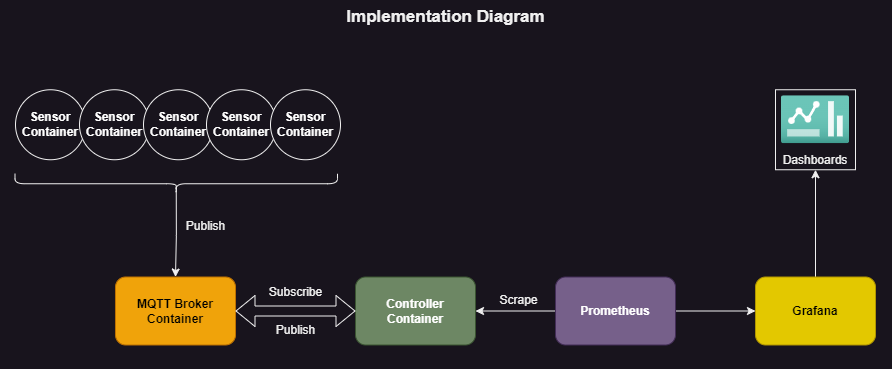
\includegraphics[scale=0.55]{implementation.png}
    \centering
    \caption{Implementation Diagram}
    \label{fig:imple_dia}
\end{figure}

\section{Dataset}
\subsection{Dataset Description}
The dataset used contains the responses of a gas multisensor device deployes on the field in an Italian city. Hourly responses averages are recorded along with gas concentrations references from a certified analyzer. The dataset contains 9357 instances of hourly averaged responses from an array of 5 metal oxide chemical sensors embedded in an Air Quality Chemical Multisensor Device. Ground Truth hourly averaged concentrations for CO, Non Metanic Hydrocarbons, Benzene, Total Nitrogen Oxides (NOx) and Nitrogen Dioxide (NO2) were provided by a co-located reference certified analyzer. Dataset can be found \href{https://www.kaggle.com/datasets/fedesoriano/air-quality-data-set/data}{here}.

\begin{table}[!h]
\begin{tabular}{|c|p{0.8\linewidth}|}
    \hline
    \multicolumn{2}{|c|}{\textbf{Attribute Information}} \\
    \hline
    \hline
    0& Date (DD/MM/YYYY) \\ \hline
    1& Time (HH.MM.SS) \\ \hline
    2& True hourly averaged concentration CO in $mg/m^3$ (reference analyzer) \\ \hline
    3& PT08.S1 (tin oxide) hourly averaged sensor response (nominally CO targeted) \\ \hline
    4& True hourly averaged overall Non Metanic HydroCarbons concentration in $microg/m^3$ (reference analyzer) \\ \hline
    5& True hourly averaged Benzene concentration in $microg/m^3$ (reference analyzer) \\ \hline
    6& PT08.S2 (titania) hourly averaged sensor response (nominally NMHC targeted) \\ \hline
    7& True hourly averaged NOx concentration in ppb (reference analyzer) \\ \hline
    8& PT08.S3 (tungsten oxide) hourly averaged sensor response (nominally NOx targeted) \\ \hline
    9& True hourly averaged NO2 concentration in $microg/m^3$ (reference analyzer) \\ \hline
    10& PT08.S4 (tungsten oxide) hourly averaged sensor response (nominally NO2 targeted) \\ \hline
    11& PT08.S5 (indium oxide) hourly averaged sensor response (nominally O3 targeted) \\ \hline
    12& Temperature in °C \\ \hline
    13& Relative Humidity (\%) \\ \hline
    14& AH Absolute Humidity  \\ \hline
\end{tabular}
\centering
\caption{Dataset Attribute Information}
\label{fig:dataset_attri}
\end{table}

\subsection{Dataset Manipulation}
Dataset was originally formatted in comma-separated values (CSV) format to be easily imported in a spreadsheet. To bring the CSV formatted dataset in a programmatically friendlier json format, a python script was developed. 
To assist with the randomized nature of data generation by the sensor simulator, for every timestamp a json object was created, with key an incremental integer and value the collection of metrics in json object format. Also empty rows were removed.

\begin{minted}[%
    framesep=2mm,
    baselinestretch=1.2,
    bgcolor=LightGray,
    fontsize=\footnotesize,
    breaklines
    ]{python}
    import csv
    import sys
    import json
    import os

    # Creates a new csv file named 'edited_csv' that doesn't contain empty rows, or rows with empty fields
    def csv_cleanup(csvfilename):
        with open(csvfilename, newline='') as csvfile:
            with open('edited_csv', 'w', newline='') as edited_csvfile:
                original = csv.reader(csvfile, delimiter=';')
                edited = csv.writer(edited_csvfile, delimiter=';')
                # fieldnames = next(original)
                # fieldnames.insert(0, "#")
                # edited.writerow(fieldnames)
                # i = 1
                for row in original:
                    if row and any(row) and any(field.strip() for field in row):
                        # row.insert(0, i)
                        edited.writerow(row)
                        # i += 1

    # Creates a json file from the edited csv file with an incremental integer as keys
    def csv_to_json(filename):
        data_dict = {}
        with open('edited_csv', newline='') as csvfile:
            edited = csv.DictReader(csvfile, delimiter=';')
            key = 1
            for row in edited: 
                data_dict[key] = row
                key += 1
        with open(filename+'.json', 'w') as jsonfile:
            jsonfile.write(json.dumps(data_dict, indent = 4))



    csvfilename = sys.argv[1]
    filename = csvfilename.split('/')[-1].split('.')[0]

    csv_cleanup(csvfilename)
    csv_to_json(filename)
    os.remove('edited_csv')
\end{minted}

The json re-formated dataset is structured as seen below.

\begin{minted}[%
    framesep=2mm,
    baselinestretch=1.2,
    bgcolor=LightGray,
    fontsize=\footnotesize,
    breaklines
    ]{json}
    {
        "1": {
            "Date": "10/03/2004",
            "Time": "18.00.00",
            "CO(GT)": "2,6",
            "PT08.S1(CO)": "1360",
            "NMHC(GT)": "150",
            "C6H6(GT)": "11,9",
            "PT08.S2(NMHC)": "1046",
            "NOx(GT)": "166",
            "PT08.S3(NOx)": "1056",
            "NO2(GT)": "113",
            "PT08.S4(NO2)": "1692",
            "PT08.S5(O3)": "1268",
            "T": "13,6",
            "RH": "48,9",
            "AH": "0,7578",
            "": ""
        },
        "2": {
            "Date": "10/03/2004",
            "Time": "19.00.00",
            "CO(GT)": "2",
            "PT08.S1(CO)": "1292",
            "NMHC(GT)": "112",
            "C6H6(GT)": "9,4",
            "PT08.S2(NMHC)": "955",
            "NOx(GT)": "103",
            "PT08.S3(NOx)": "1174",
            "NO2(GT)": "92",
            "PT08.S4(NO2)": "1559",
            "PT08.S5(O3)": "972",
            "T": "13,3",
            "RH": "47,7",
            "AH": "0,7255",
            "": ""
        }
    }
\end{minted}

\section{Sensor Simulator}
\subsection{Scenario}
The sensors remain in a low-power idle state to conserve energy. They are subscribed to the "collect-data" topic but are not actively collecting or publishing data. The controller node publishes a message to the MQTT topic "collect-data". This message is broadcast to all subscribed sensors by the MQTT broker. Upon receiving the trigger from the collect-data topic, sensors begin collecting air quality metrics. After collecting the data, each sensor publishes its metrics to its respective MQTT topic and returns to an idle state.
\subsection{Application}
As described on the scenario, first action on the application is establishing a connection to the MQTT broker, making sure to reconnect in case of disconnection, which would happen often in a real case scenario utilizing an unreliable cellular connection and subscribing to the "collect-data" topic. Then, once a message from the topic is received the data collection and publishing script is executed.

\begin{minted}[%
    framesep=2mm,
    baselinestretch=1.2,
    bgcolor=LightGray,
    fontsize=\footnotesize,
    breaklines
    ]{python}
    import socket
    import time
    import subprocess
    import paho.mqtt.client as mqtt_client

    port = 1883  # Default port for MQTT communication
    topic = "collect-data"  # Topic to subscribe to for data collection
    hostname = socket.gethostname()  # Get the hostname of the machine running this script. Machine (container) hostname is enforced later-on by docker compose 
    client_id = 'subscribe-{}'.format(hostname)  # Unique client ID for MQTT connection
    # broker = 'localhost'  # Uncomment this line for local broker testing
    broker = 'host.docker.internal'  # Use when running in a Docker environment

    def connect_mqtt():
        """
        Connects to the MQTT broker and sets up event handlers for connect, disconnect, and message events.
        """

        def on_connect(client, userdata, flags, rc):
            """
            Callback triggered upon connecting to the MQTT broker.
            """
            if rc == 0:
                print("Connected to MQTT Broker!")
                client.subscribe(topic)  # Subscribe to the specified topic
            else:
                print("Failed to connect, return code %d\n", rc)
        
        def on_disconnect(client, userdata, rc):
            """
            Callback triggered when the MQTT client disconnects from the broker.
            Implements an exponential backoff strategy for reconnection attempts.
            """
            FIRST_RECONNECT_DELAY = 1
            RECONNECT_RATE = 2
            MAX_RECONNECT_COUNT = 12
            MAX_RECONNECT_DELAY = 60

            print("Disconnected with result code: %s", rc)
            reconnect_count, reconnect_delay = 0, FIRST_RECONNECT_DELAY
            while reconnect_count < MAX_RECONNECT_COUNT:
                print("Reconnecting in {} seconds...".format(reconnect_delay))
                time.sleep(reconnect_delay)

                try:
                    client.reconnect()
                    print("Reconnected successfully!")
                    return
                except Exception as err:
                    print("{}. Reconnect failed. Retrying...".format(err))

                reconnect_delay *= RECONNECT_RATE
                reconnect_delay = min(reconnect_delay, MAX_RECONNECT_DELAY)
                reconnect_count += 1
            print("Reconnect failed after {} attempts. Exiting...".format(reconnect_count))

        def on_message(client, userdata, msg):
            """
            Callback triggered when a message is received on the subscribed topic.
            """
            print("Received `{}` from `{}` topic".format(msg.payload.decode(), msg.topic))
            subprocess.run(["./sensor_data"])  # Execute the sensor_data script upon message receipt

        # Create an MQTT client instance, assign the callback functions and connect
        client = mqtt_client.Client(client_id)
        client.on_connect = on_connect
        client.on_disconnect = on_disconnect
        client.on_message = on_message
        client.connect(broker, port)
        return client  # Return the configured client instance

    def run():
        """
        Main function to connect the MQTT client and start its loop.
        """
        client = connect_mqtt()
        client.loop_forever()

    if __name__ == '__main__':
        run()
\end{minted}

The data collection script, again starts by establishing a connection client with the MQTT broker. Once connection is established, the data collection process starts. To simulate a real-world scenario, to add variation between the multiple sensors and a randomization element, that also prolongs the use of the dataset before going over the same data, an elaborate process was devised. To ensure the randomized data have a real-world, logical flow, the next data point is selected from the range (previous - 2, previous + 3). This ensures that the metrics collected each time are only a few hours apart instead of completely random, which would result in completely abnormal differences on metrics that wouldn't be observed on metrics taken a few minutes or an hour apart. It also ensures that the data point slowly moves forward in time, as to not overly repeat the same data. The starting point for this process is randomized using another script, to ensure results between sensors don't overlap heavily. Since the data collection process is ephemeral, the data points needs to be stored. This could have been achieved in a number of ways, like passing it back and forth between the main subscription script or using an environmental variable, but storing to a file was preferred as it could also be utilized if a recovery scenario was to be covered. Once the end of the database is reached, a new starting point is, again, randomly selected.

\begin{minted}[%
    framesep=2mm,
    baselinestretch=1.2,
    bgcolor=LightGray,
    fontsize=\footnotesize,
    breaklines
    ]{python}
    import json
    import random, os
    import socket
    import subprocess
    from dotenv import load_dotenv
    import paho.mqtt.client as mqtt_client

    port = 1883  # Default port for MQTT communication
    hostname = socket.gethostname()  # Retrieve the hostname of the current machine. Hostname is enforced by docker compose.
    topic = "sensor-data/{}".format(hostname)  # Define the unique topic for publishing sensor data
    client_id = 'publish-{}'.format(hostname)  # Unique client ID for MQTT connection
    # broker = 'localhost'  # Uncomment this line for local broker testing
    broker = 'host.docker.internal'  # Use this broker when running in a Docker environment

    def connect_mqtt():
        """
        Connects to the MQTT broker and sets up the on_connect callback.
        """

        def on_connect(client, userdata, flags, rc):
            """
            Callback triggered upon connecting to the MQTT broker.
            """
            if rc == 0:
                print("Connected to MQTT Broker!")
            else: 
                print("Failed to connect, return code %d\n", rc)

        client = mqtt_client.Client(client_id)
        client.on_connect = on_connect 
        client.connect(broker, port)  
        return client  

    def data_gen():
        """
        Generates sensor data by selecting a random entry from a dataset.
        The selection point is controlled via an environment variable.
        """
        with open("dataset.json") as datafile:
            json_data = json.load(datafile)  # Load the dataset from the JSON file
        
            load_dotenv()  # Load environment variables from the .env file
            startpoint = int(os.getenv('STARTPOINT'))  # Get the STARTPOINT from the .env file
            # Randomize the data selection around the startpoint. Slowly moves forward in time, while keeping results semi-random and ensuring a logical history.
            randomizer = random.randint(startpoint - 2, startpoint + 3)
            while randomizer not in range(1, len(json_data)):  # Ensure the randomizer is valid
                subprocess.run(["./set_startpoint"])  # Run a script to reset the startpoint
                load_dotenv()  # Reload environment variables
                startpoint = int(os.getenv('STARTPOINT'))
                randomizer = random.randint(startpoint - 10, startpoint + 10)

            # Update the STARTPOINT in the .env file
            with open(".env", "w") as f:
                f.write("STARTPOINT={}".format(randomizer))

            randata = json_data[str(randomizer)]  # Fetch the random data entry
            return randata  # Return the selected data

    def publish(client, data):
        """
        Publishes a message to the MQTT topic.
        """
        msg = str(data)  # Convert the data to a string
        result = client.publish(topic, msg)  # Publish the message to the topic
        status = result[0]  # Check the result status
        if status == 0:
            print("Sent `{}` to topic `{}`".format(msg, topic))
        else:
            print("Failed to send message to topic {}".format(topic))        

    if __name__ == '__main__':
        client = connect_mqtt()  # Establish the MQTT connection
        client.loop_start()  # Start the MQTT client loop in a separate thread
        randata = data_gen()  # Generate random sensor data
        publish(client, randata)  # Publish the generated data to the topic
        client.loop_stop()  # Stop the MQTT client loop
\end{minted}

\begin{minted}[%
    framesep=2mm,
    baselinestretch=1.2,
    bgcolor=LightGray,
    fontsize=\footnotesize,
    breaklines
    ]{python}
    import json, random

    def set_startpoint():
        """
        Sets a STARTPOINT value based on the dataset's size and writes it to an .env file.
        """
        with open("dataset.json") as datafile:
            json_data = json.load(datafile) # Load the dataset from a JSON file
            
            endpoint = round(len(json_data)/10) # Determine the upper limit for the STARTPOINT range
            startpoint = str(random.randint(1, endpoint))

            print("Setting STARTPOINT as {}".format(startpoint))

            with open(".env", "w") as f:
                f.write("STARTPOINT={}".format(startpoint)) # Write the STARTPOINT to the .env file

    if __name__ == '__main__':
        set_startpoint()
\end{minted}

Only libraries required, are "paho-mqtt" and "python-dotenv".

\subsection{Containerization}
IoT sensors usually are embedded on microcontrollers with limited hardware resources. While minimal, optimized subsets of Python do exist, building the Python scripts and using the binaries directly, makes more sense. To stick with the minimal, lightweight enviroment expected in an IoT microcontroller, a minimal linux docker image as base is a good fit. The \href{https://hub.docker.com/_/alpine/}{Alpine docker image} was selected, as it is the industry standard for minimal, striped down Linux images, and current latest ones are only around 5MB uncompressed. To build the Python scripts PyInstaller was used, but because Alpine utilizes \href{https://musl.libc.org/}{Musl C library}, instead of the \href{https://www.gnu.org/software/libc/}{GNU C library}, a third party PyInstaller-ready, Alpine-based Python image was used, that can be found \href{https://github.com/six8/pyinstaller-alpine}{here}. Using this image also removes the requirement of installing PyInstaller, a great example of how docker removes environmental dependencies. The following command was used:
\begin{minted}[%
    framesep=2mm,
    baselinestretch=1.2,
    bgcolor=LightGray,
    fontsize=\footnotesize,
    breaklines
    ]{bash}
    $ docker run --rm -v "${PWD}:/src" anastzampetis/pyinstaller-alpine --noconfirm --onefile --log-level DEBUG --clean <script_name>.py
\end{minted}
Once the binaries were built, a simple Dockerfile was used to copy the binaries and the json formated dataset into the base Alpine image and set the binaries to be executed when running the container.
\begin{minted}[%
    framesep=2mm,
    baselinestretch=1.2,
    bgcolor=LightGray,
    fontsize=\footnotesize,
    breaklines
    ]{dockerfile}
    FROM alpine

    WORKDIR /app
    ADD dist/sensor_data .
    ADD dist/sensor_sub .
    ADD dist/set_startpoint .
    ADD dataset.json .

    CMD ./set_startpoint && ./sensor_sub
\end{minted}  
Finally to build the image, below command was executed:
\begin{minted}[%
    framesep=2mm,
    baselinestretch=1.2,
    bgcolor=LightGray,
    fontsize=\footnotesize,
    breaklines
    ]{bash}
    $ docker build -t anastzampetis/sensor-emul:latest -f Dockerfile .
\end{minted}

\begin{figure}[!h]
    \graphicspath{ {./screenshots/} }
    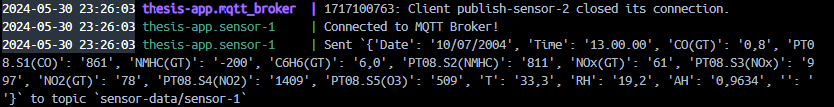
\includegraphics[width=1\textwidth]{sensor-log.png}
    \centering
    \caption{Output log of the simulated sensor }
    \label{fig:sensor_log}
\end{figure}

\section{MQTT Broker}
For the MQTT broker, the Eclipse Mosquitto MQTT broker was selected. Mosquitto is an open-source message broker that implements the MQTT protocol. Mosquitto is designed to be small and efficient, suitable for IoT devices with constrained resources, and fits well in a microservice enviroment. It's also very capable of handling even large-scale deployments, making it a good fit for a scalable enviroment.

To stay true to a microservice architecture and to make deployment and management easier, the Mosquitto MQTT broker was deployed in a docker container. It is already available in an official image found \href{https://hub.docker.com/_/eclipse-mosquitto}{here}. Configuring the container was simple in the scope of this implementation, since there was no need for secutiry protocols and persisting data inside the broker container because Prometheus is utilized.

\begin{minted}[%
    framesep=2mm,
    baselinestretch=1.2,
    bgcolor=LightGray,
    fontsize=\footnotesize,
    breaklines
    ]{bash}
    persistence false     # No need to persist data, since it's pushed to Prometheus
    listener 1883         # The listener port that clients publish to
    allow_anonymous true  # Since there is no need for security, anonymous is allowed.
\end{minted}

\section{Controller Node}
The controller node serves a number of important functions. Firstly, it's responsible for publishing on the "collect-data" MQTT topic, so the sensor simulators will leave the idle state and collect the data. Then, by subscribing to the topics the sensors publish to, "sensor-data/\#" (usign a wildcard topic definition also allows for scaling of sensors), the controller node will receive messages from each topic, containing the sensor data.

Once these messages are received, using the "prometheus\_client" library all metrics are converted in Prometheus format and exposed to an endpoint. Every metric is assigned to a different Gauge type Prometheus metric and labeled usign the sensor unique id. A gauge is a metric that represents a single numerical value that can arbitrarily go up and down. This part of the controller's functionality is essensially a Prometheus exporter.

Usually Prometheus exporters collect data periodically, but continiously expose last collected metrics on an HTTP endpoint. In this case, thought, to make it easier to change the rate of data collection, by changing the scraping rate of Prometheus, a different design was implemented. The controller, utilizing the "fastapi" library and "gunicorn" exposes an API endpoint. When Prometheus scrapes this endpoint, the data collection process is triggered by the controller, and after a small time delay the controller respondes with the metrics. Implementation is split between a main script and two modules.

\begin{minted}[%
    framesep=2mm,
    baselinestretch=1.2,
    bgcolor=LightGray,
    fontsize=\footnotesize,
    breaklines
    ]{python}
    import time
    from fastapi import FastAPI, Response
    from prometheus_client import generate_latest
    from exporter_func import *

    app = FastAPI(debug=False)

    # Define an endpoint to serve metrics
    @app.get("/metrics")
    def get_metrics_app():
        start_time = time.time()
        
        # Connect to MQTT and start collecting data
        sub_client = connect_sub_mqtt()
        sub_client.loop_start()
        gather_data()
        time.sleep(1) # Allow time for data collection, in case sensors take time to respond
        sub_client.loop_stop()

        # Generate metrics data in Prometheus format
        data = generate_latest()

        end_time = time.time()
        execution_time = end_time - start_time
        print("Execution time:",execution_time)

        # Return the metrics data as a plain text HTTP response
        return Response(content=data, media_type="text/plain")

    # Define a root endpoint with a simple message
    @app.get("/")
    async def root():
        return "Go to /metrics for gitlab metrics"

    # Note for running the application locally
    # Use the command:
    # gunicorn -b localhost:8000 exporter:app -k uvicorn.workers.UvicornWorker
\end{minted}

\begin{minted}[%
    framesep=2mm,
    baselinestretch=1.2,
    bgcolor=LightGray,
    fontsize=\footnotesize,
    breaklines
    ]{python}
    import paho.mqtt.client as mqtt_client
    import json, time
    from exporter_var import *

    # Function to establish a connection to the MQTT broker and subscribe to a topic
    def connect_sub_mqtt():

        # Callback for successful connection to the MQTT broker
        def on_connect(client, userdata, flags, rc):
            if rc == 0:
                print("Connected to MQTT Broker!")
                client.subscribe(sub_topic) # Subscribe to the specified topic
            else:
                print("Failed to connect, return code %d\n", rc)
        
        # Callback for handling disconnection from the MQTT broker
        def on_disconnect(client, userdata, rc):

            FIRST_RECONNECT_DELAY = 1
            RECONNECT_RATE = 2
            MAX_RECONNECT_COUNT = 12
            MAX_RECONNECT_DELAY = 60

            print("Disconnected with result code: %s", rc)
            reconnect_count, reconnect_delay = 0, FIRST_RECONNECT_DELAY
            while reconnect_count < MAX_RECONNECT_COUNT:
                print("Reconnecting in {} seconds...".format(reconnect_delay))
                time.sleep(reconnect_delay)

                try:
                    client.reconnect()
                    print("Reconnected successfully!")
                    return
                except Exception as err:
                    print("{}. Reconnect failed. Retrying...".format(err))

                reconnect_delay *= RECONNECT_RATE # Increase delay exponentially
                reconnect_delay = min(reconnect_delay, MAX_RECONNECT_DELAY)
                reconnect_count += 1
            print("Reconnect failed after {} attempts. Exiting...".format(reconnect_count))

        # Callback for receiving messages from the MQTT broker
        def on_message(client, userdata, msg):

            print("Received data from `{}` topic".format(msg.topic))
            promethify_data(msg)  # Process the received message for Prometheus metrics

        # Initialize the MQTT client and assign the callbacks
        client = mqtt_client.Client(sub_client_id)
        client.on_connect = on_connect
        client.on_disconnect = on_disconnect
        client.on_message = on_message
        client.connect(broker, sub_port)
        return client

    # Function to continuously run the MQTT subscriber
    def sub_client_run():
        sub_client = connect_sub_mqtt()
        sub_client.loop_forever()

    # Function to publish a request message to collect data
    def request_data(client):
        msg = 'Time to collect data.'
        result = client.publish(pub_topic, msg)
        status = result[0]
        if status == 0:
            print("Sent `{}` to topic `{}`".format(msg, pub_topic))
        else:
            print("Failed to send message to topic {}".format(pub_topic))

    # Function to connect to the MQTT broker as a publisher
    def connect_pub_mqtt():

        def on_connect(client, userdata, flags, rc):
            if rc == 0:
                print("Connected to MQTT Broker!")
            else:
                print("Failed to connect, return code %d\n", rc)

        client = mqtt_client.Client(pub_client_id)
        client.on_connect = on_connect
        client.connect(broker, pub_port)
        return client

    # Function to gather data by publishing a request message
    def gather_data():
        pub_client = connect_pub_mqtt()
        pub_client.loop_start()
        request_data(pub_client)
        pub_client.loop_stop()

    # Function to assign received data to Prometheus metrics
    def assign_data(prom_var, data_name, sensor, jsondata):

        value =  float(jsondata[data_name].replace(',', '.')) # Parse the value
        if  value != -200:  # Exclude no readings
            prom_var.labels(sensor).set(value) # Set the metric value with sensor label  

    # Function to process received MQTT messages and update Prometheus metrics
    def promethify_data(msg):

        sensor = msg.topic.split('/')[1] # Extract sensor name from topic
        # Decode and parse the JSON payload
        jsondata_string = msg.payload.decode().replace("'", '"') 
        jsondata = json.loads(jsondata_string)

        # Assign each metric to the corresponding Prometheus variable
        assign_data(air_quality_co_gt_gauge, "CO(GT)", sensor, jsondata)
        assign_data(air_quality_pt08s1_co_gauge, "PT08.S1(CO)", sensor, jsondata)
        assign_data(air_quality_nmhc_gt_gauge, "NMHC(GT)", sensor, jsondata)
        assign_data(air_quality_c6h6_gt_gauge, "C6H6(GT)", sensor, jsondata)
        assign_data(air_quality_pt08s2_nmhc_gauge, "PT08.S2(NMHC)", sensor, jsondata)
        assign_data(air_quality_nox_gt_gauge, "NOx(GT)", sensor, jsondata)
        assign_data(air_quality_pt08s3_nox_gauge, "PT08.S3(NOx)", sensor, jsondata)
        assign_data(air_quality_no2_gt_gauge, "NO2(GT)", sensor, jsondata)
        assign_data(air_quality_pt08s4_no2_gauge, "PT08.S4(NO2)", sensor, jsondata)
        assign_data(air_quality_pt08s5_o3_gauge, "PT08.S5(O3)", sensor, jsondata)
        assign_data(air_quality_t_gauge, "T", sensor, jsondata)
        assign_data(air_quality_rh_gauge, "RH", sensor, jsondata)
        assign_data(air_quality_ah_gauge, "AH", sensor, jsondata)
\end{minted}

\begin{minted}[%
    framesep=2mm,
    baselinestretch=1.2,
    bgcolor=LightGray,
    fontsize=\footnotesize,
    breaklines
    ]{python}
    from prometheus_client import Gauge

    sub_port = 1883 # Port for the subscriber
    pub_port = 1883 # Port for the publisher
    sub_topic = "sensor-data/#" # Subscription topic for sensor data (wildcard for all subtopics)
    pub_topic = "collect-data" # Topic to publish data collection requests
    sub_client_id = 'subscribe-exporter' # Client ID for the MQTT subscriber
    pub_client_id = 'publish-exporter' # Client ID for the MQTT publisher
    #broker = 'localhost' # uncomment for local testing
    broker = 'host.docker.internal' # Docker-specific hostname for connecting to the broker


    # Prometheus metrics definitions
    # Each metric is defined as a Prometheus Gauge with a description and a label for 'sensor'

    air_quality_co_gt_gauge = Gauge('air_quality_co_gt_gauge', 'True hourly averaged concentration CO in mg/m^3 (reference analyzer)', ['sensor'])

    air_quality_pt08s1_co_gauge = Gauge('air_quality_pt08s1_co_gauge', 'Tin oxide hourly averaged sensor response (nominally CO targeted)', ['sensor'])

    air_quality_nmhc_gt_gauge = Gauge('air_quality_nmhc_gt_gauge', 'True hourly averaged overall Non Metanic HydroCarbons concentration in microg/m^3 (reference analyzer)', ['sensor'])

    air_quality_c6h6_gt_gauge = Gauge('air_quality_c6h6_gt_gauge', 'True hourly averaged Benzene concentration in microg/m^3 (reference analyzer)', ['sensor'])

    air_quality_pt08s2_nmhc_gauge = Gauge('air_quality_pt08s2_nmhc_gauge', 'Titania hourly averaged sensor response (nominally NMHC targeted)', ['sensor'])

    air_quality_nox_gt_gauge = Gauge('air_quality_nox_gt_gauge', 'True hourly averaged NOx concentration in ppb (reference analyzer)', ['sensor'])

    air_quality_pt08s3_nox_gauge = Gauge('air_quality_pt08s3_nox_gauge', 'Tungsten oxide hourly averaged sensor response (nominally NOx targeted)', ['sensor'])

    air_quality_no2_gt_gauge = Gauge('air_quality_no2_gt_gauge', 'True hourly averaged NO2 concentration in microg/m^3 (reference analyzer)', ['sensor'])

    air_quality_pt08s4_no2_gauge = Gauge('air_quality_pt08s4_no2_gauge', 'Tungsten oxide hourly averaged sensor response (nominally NO2 targeted)', ['sensor'])

    air_quality_pt08s5_o3_gauge = Gauge('air_quality_pt08s5_o3_gauge', 'Indium oxide hourly averaged sensor response (nominally O3 targeted)', ['sensor'])

    air_quality_t_gauge = Gauge('air_quality_t_gauge', 'Temperature in C', ['sensor'])

    air_quality_rh_gauge = Gauge('air_quality_rh_gauge', 'Relative Humidity (%)', ['sensor'])

    air_quality_ah_gauge = Gauge('air_quality_ah_gauge', 'Absolute Humidity', ['sensor'])
\end{minted}

Final output of the scripts on the endpoint that Prometheus scrapes is the Prometheus formated metrics and can be seen in an example below.

\begin{minted}[%
    framesep=2mm,
    baselinestretch=1.2,
    bgcolor=LightGray,
    fontsize=\footnotesize,
    breaklines
    ]{bash}
    # HELP air_quality_co_gt_gauge True hourly averaged concentration CO in mg/m^3 (reference analyzer)
    # TYPE air_quality_co_gt_gauge gauge
    air_quality_co_gt_gauge{sensor="sensor-5"} 4.6
    air_quality_co_gt_gauge{sensor="sensor-1"} 2.7
    air_quality_co_gt_gauge{sensor="sensor-2"} 2.1
    air_quality_co_gt_gauge{sensor="sensor-3"} 4.3
    air_quality_co_gt_gauge{sensor="sensor-4"} 1.9
    # HELP air_quality_pt08s1_co_gauge Tin oxide hourly averaged sensor response (nominally CO targeted)
    # TYPE air_quality_pt08s1_co_gauge gauge
    air_quality_pt08s1_co_gauge{sensor="sensor-5"} 1808.0
    air_quality_pt08s1_co_gauge{sensor="sensor-1"} 1280.0
    air_quality_pt08s1_co_gauge{sensor="sensor-2"} 1327.0
    air_quality_pt08s1_co_gauge{sensor="sensor-3"} 1559.0
    air_quality_pt08s1_co_gauge{sensor="sensor-4"} 1096.0
    # HELP air_quality_nmhc_gt_gauge True hourly averaged overall Non Metanic HydroCarbons concentration in microg/m^3 (reference analyzer)
    # TYPE air_quality_nmhc_gt_gauge gauge
    air_quality_nmhc_gt_gauge{sensor="sensor-5"} 262.0
    air_quality_nmhc_gt_gauge{sensor="sensor-1"} 122.0
    air_quality_nmhc_gt_gauge{sensor="sensor-2"} 256.0
    air_quality_nmhc_gt_gauge{sensor="sensor-3"} 535.0
    air_quality_nmhc_gt_gauge{sensor="sensor-4"} 220.0
    # HELP air_quality_c6h6_gt_gauge True hourly averaged Benzene concentration in microg/m^3 (reference analyzer)
    # TYPE air_quality_c6h6_gt_gauge gauge
    air_quality_c6h6_gt_gauge{sensor="sensor-5"} 20.6
    air_quality_c6h6_gt_gauge{sensor="sensor-1"} 9.6
    air_quality_c6h6_gt_gauge{sensor="sensor-2"} 9.8
    air_quality_c6h6_gt_gauge{sensor="sensor-3"} 18.9
    air_quality_c6h6_gt_gauge{sensor="sensor-4"} 9.2
    # HELP air_quality_pt08s2_nmhc_gauge Titania hourly averaged sensor response (nominally NMHC targeted)
    # TYPE air_quality_pt08s2_nmhc_gauge gauge
    air_quality_pt08s2_nmhc_gauge{sensor="sensor-5"} 1312.0
    air_quality_pt08s2_nmhc_gauge{sensor="sensor-1"} 964.0
    air_quality_pt08s2_nmhc_gauge{sensor="sensor-2"} 971.0
    air_quality_pt08s2_nmhc_gauge{sensor="sensor-3"} 1267.0
    air_quality_pt08s2_nmhc_gauge{sensor="sensor-4"} 947.0
    # HELP air_quality_nox_gt_gauge True hourly averaged NOx concentration in ppb (reference analyzer)
    # TYPE air_quality_nox_gt_gauge gauge
    air_quality_nox_gt_gauge{sensor="sensor-5"} 261.0
    air_quality_nox_gt_gauge{sensor="sensor-1"} 193.0
    air_quality_nox_gt_gauge{sensor="sensor-2"} 124.0
    air_quality_nox_gt_gauge{sensor="sensor-3"} 230.0
    air_quality_nox_gt_gauge{sensor="sensor-4"} 115.0
    # HELP air_quality_pt08s3_nox_gauge Tungsten oxide hourly averaged sensor response (nominally NOx targeted)
    # TYPE air_quality_pt08s3_nox_gauge gauge
    air_quality_pt08s3_nox_gauge{sensor="sensor-5"} 753.0
    air_quality_pt08s3_nox_gauge{sensor="sensor-1"} 963.0
    air_quality_pt08s3_nox_gauge{sensor="sensor-2"} 803.0
    air_quality_pt08s3_nox_gauge{sensor="sensor-3"} 653.0
    air_quality_pt08s3_nox_gauge{sensor="sensor-4"} 872.0
    # HELP air_quality_no2_gt_gauge True hourly averaged NO2 concentration in microg/m^3 (reference analyzer)
    # TYPE air_quality_no2_gt_gauge gauge
    air_quality_no2_gt_gauge{sensor="sensor-5"} 157.0
    air_quality_no2_gt_gauge{sensor="sensor-1"} 113.0
    air_quality_no2_gt_gauge{sensor="sensor-2"} 89.0
    air_quality_no2_gt_gauge{sensor="sensor-3"} 149.0
    air_quality_no2_gt_gauge{sensor="sensor-4"} 113.0
    # HELP air_quality_pt08s4_no2_gauge Tungsten oxide hourly averaged sensor response (nominally NO2 targeted)
    # TYPE air_quality_pt08s4_no2_gauge gauge
    air_quality_pt08s4_no2_gauge{sensor="sensor-5"} 1993.0
    air_quality_pt08s4_no2_gauge{sensor="sensor-1"} 1544.0
    air_quality_pt08s4_no2_gauge{sensor="sensor-2"} 1705.0
    air_quality_pt08s4_no2_gauge{sensor="sensor-3"} 2047.0
    air_quality_pt08s4_no2_gauge{sensor="sensor-4"} 1519.0
    # HELP air_quality_pt08s5_o3_gauge Indium oxide hourly averaged sensor response (nominally O3 targeted)
    # TYPE air_quality_pt08s5_o3_gauge gauge
    air_quality_pt08s5_o3_gauge{sensor="sensor-5"} 1698.0
    air_quality_pt08s5_o3_gauge{sensor="sensor-1"} 1285.0
    air_quality_pt08s5_o3_gauge{sensor="sensor-2"} 1120.0
    air_quality_pt08s5_o3_gauge{sensor="sensor-3"} 1373.0
    air_quality_pt08s5_o3_gauge{sensor="sensor-4"} 684.0
    # HELP air_quality_t_gauge Temperature in C
    # TYPE air_quality_t_gauge gauge
    air_quality_t_gauge{sensor="sensor-5"} 18.4
    air_quality_t_gauge{sensor="sensor-1"} 9.5
    air_quality_t_gauge{sensor="sensor-2"} 21.6
    air_quality_t_gauge{sensor="sensor-3"} 15.7
    air_quality_t_gauge{sensor="sensor-4"} 18.6
    # HELP air_quality_rh_gauge Relative Humidity (%)
    # TYPE air_quality_rh_gauge gauge
    air_quality_rh_gauge{sensor="sensor-5"} 41.7
    air_quality_rh_gauge{sensor="sensor-1"} 64.1
    air_quality_rh_gauge{sensor="sensor-2"} 41.7
    air_quality_rh_gauge{sensor="sensor-3"} 62.5
    air_quality_rh_gauge{sensor="sensor-4"} 36.9
    # HELP air_quality_ah_gauge Absolute Humidity
    # TYPE air_quality_ah_gauge gauge
    air_quality_ah_gauge{sensor="sensor-5"} 0.8732
    air_quality_ah_gauge{sensor="sensor-1"} 0.7597
    air_quality_ah_gauge{sensor="sensor-2"} 1.0606
    air_quality_ah_gauge{sensor="sensor-3"} 1.1092
    air_quality_ah_gauge{sensor="sensor-4"} 0.7829
\end{minted}

To package the controller node application in a docker image, a simple Dockerfile was used. Using the official Python 3.11 image as base, all python modules are copied in the image along with the requirements file in order to install dependencies. After installing the dependencies and exposing one port for communication with the MQTT broker and one for the Prometheus metrics endpoint, the application is ready to run inside the container. An entrypoint was set to run the application using Gunicorn with Uvicorn workers.

\begin{minted}[%
    framesep=2mm,
    baselinestretch=1.2,
    bgcolor=LightGray,
    fontsize=\footnotesize,
    breaklines
    ]{dockerfile}
    FROM python:3.11.0

    # Set the working directory inside the container
    WORKDIR /srv/exporter

    # Add the main application and supporting scripts to the working directory
    ADD exporter.py /srv/exporter/
    ADD exporter_func.py /srv/exporter/
    ADD exporter_var.py /srv/exporter/
    ADD requirements.txt /srv/exporter/

    # Set execute permissions for all users on the project directory
    RUN chmod -R a+x /srv/exporter

    # Install the Python dependencies specified in requirements.txt
    RUN python3 -m pip install -r requirements.txt

    # Expose the necessary ports for the Prometheus metrics endpoint and the MQTT protocol
    EXPOSE 8000
    EXPOSE 1883

    # Set the entrypoint command to run the application using Gunicorn with Uvicorn workers
    ENTRYPOINT [ "gunicorn", "-b", "0.0.0.0:8000", "exporter:app", "-k", "uvicorn.workers.UvicornWorker" ]
\end{minted}

\section{Prometheus}
Setting up Prometheus is made extrememely easy, thanks to the usage of containers and the pre-build docker images available. Since Prometheus is such a widely used metrics collector and usually a core component of every observability stack, a lot of different images exist.

Usually, the difference in these images are the base images used, additional features and functionalities provided, or the time it takes for updates on source to be made available on the image. In this implementation the official image was used, prom/prometheus, which can be found \href{https://hub.docker.com/r/prom/prometheus}{here}.

Using this image, only a configuration yaml file and a few deployment flags need to be provided when starting the Prometheus container. The configuration file can contain an extensive list of settings, providing substansial granularity, but in most cases, such as in this implementation, only a few settings are crucial. These settings usually are some global configurations like scrape interval or scrape timeout and the scrape configurations that are organised in jobs. Each job can have it's own settings that override the global ones but must have at least one scrape targets. Scrape targers are the endpoints that Prometheus scrapes and can either be set statically, as it is done for this case, or dynamically and targets are automatically detected using Prometheus's Service Discovery.

Prometheus graphical user interface can be access on <hosts\_ip\_address>:9090

\begin{figure}[!h]
    \graphicspath{ {./screenshots/} }
    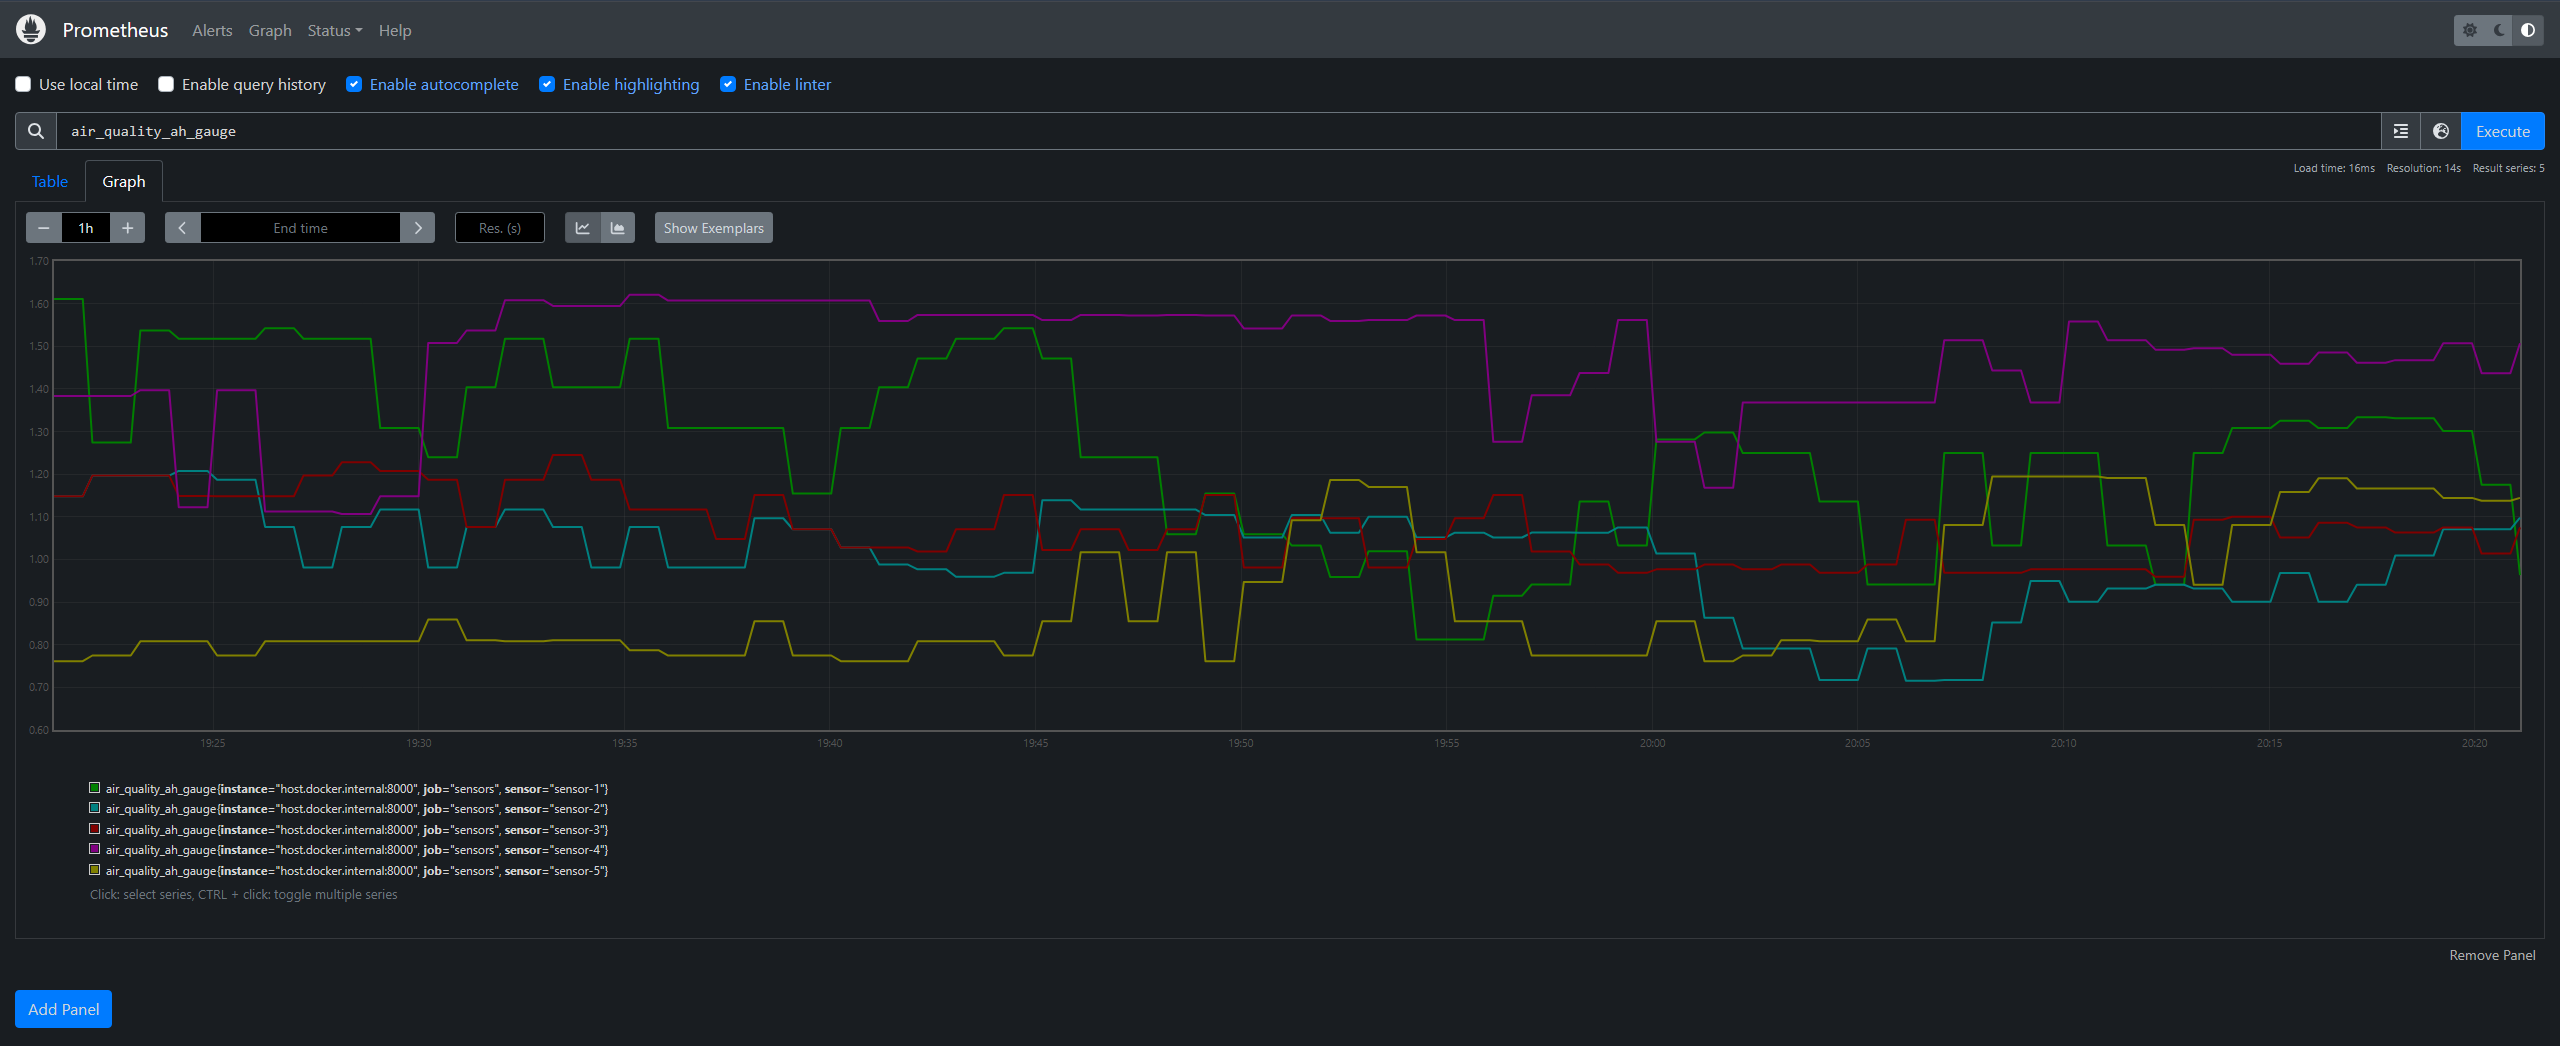
\includegraphics[width=1\textwidth]{prometheus-graph.png}
    \centering
    \caption{Simple graphing options on Prometheus UI}
    \label{fig:prom_graph}
\end{figure}

\begin{figure}[!h]
    \graphicspath{ {./screenshots/} }
    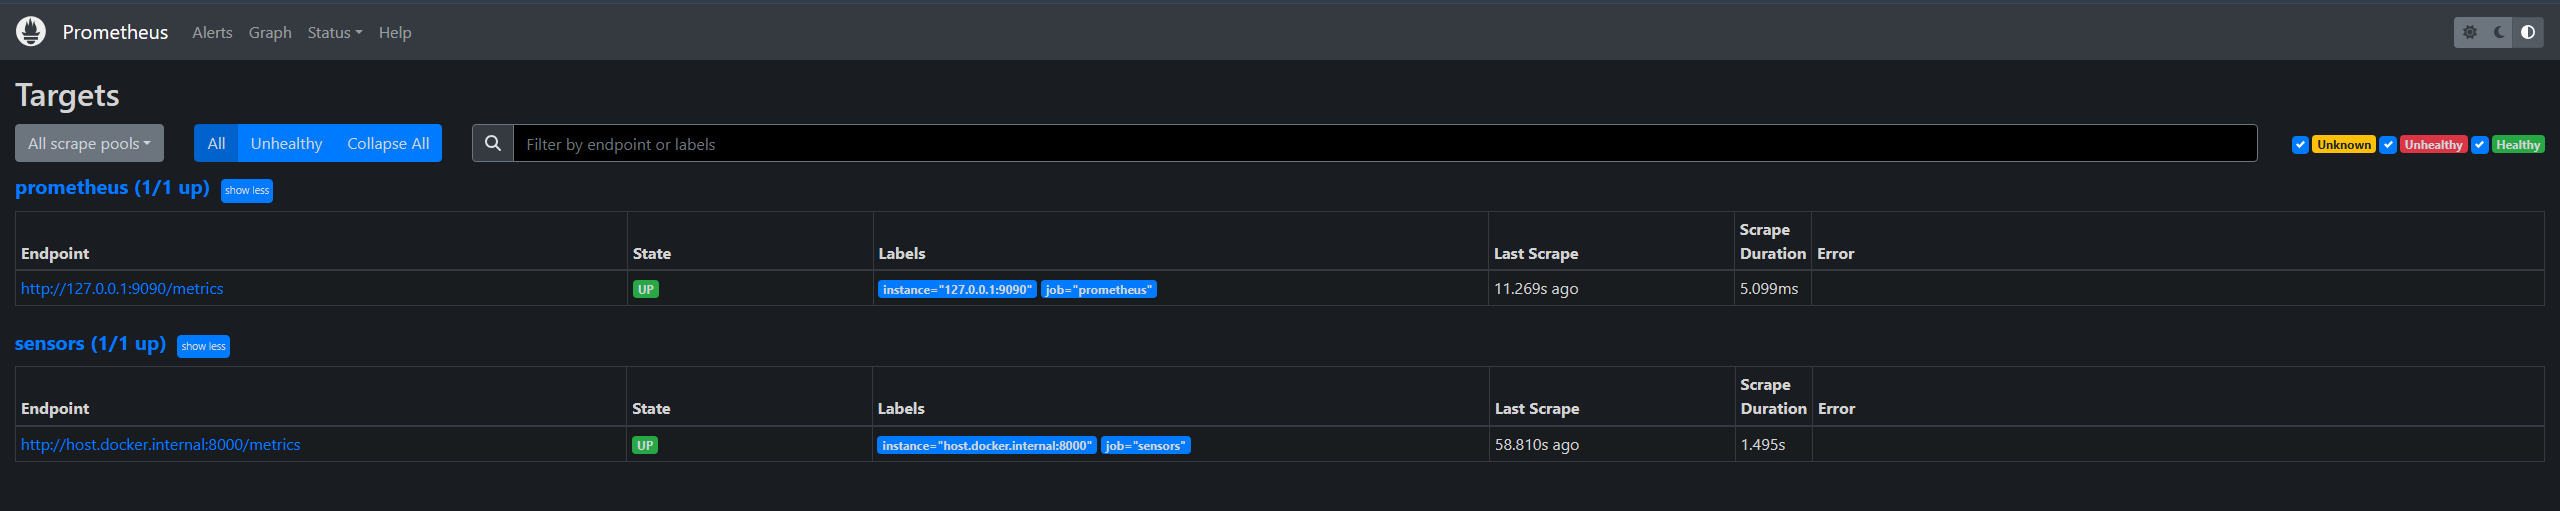
\includegraphics[width=1\textwidth]{prometheus-targets.png}
    \centering
    \caption{Prometheus targets UI overview}
    \label{fig:prom_targets}
\end{figure}

\begin{minted}[%
    framesep=2mm,
    baselinestretch=1.2,
    bgcolor=LightGray,
    fontsize=\footnotesize,
    breaklines
    ]{yaml}
    global:
    scrape_interval:     15s
    evaluation_interval: 15s

    rule_files:
    - prometheus_alerts_rules.yml

    scrape_configs:

    - job_name: prometheus # Collecting data from Prometheus itself
        static_configs:
        - targets: ['127.0.0.1:9090']

    - job_name: sensors # Collecting metrics from the Controller Node
        scrape_interval: 60s
        scrape_timeout: 50s
        static_configs:
        - targets: ['host.docker.internal:8000'] # Using host.docker.internal to direct containerized prometheus to host's 127.0.0.1 (localhost)
\end{minted}

Some very important configuration settings are passed to the Prometheus container as flags when starting it. To be able to refresh configuration without restarting the whole container, configuration yamls are mounted onto the container from local storage, to make it easy to manipulate them, and the "--web.enable-lifecycle" flag is set. This enables users to update Prometheus configuration, to add additional scrape targets for example, by changing the config files and using Prometheus REST API to reload Prometheus. Also, to properly store the time-series database (TSDB), a host storage directory was mounted on the internal container storage directory. This ensures data integrity in case the containers crashes, or is stopped or deleted. Finally, using the "--storage.tsdb.retention.time" flag data retention time was set to one year.

\section{Grafana}
\subsection{Container setup}
Setting up Grafana in a container is even simpler than Prometheus, since no configuration is needed when using the \href{official Grafana docker image}{https://hub.docker.com/r/grafana/grafana}.
Other than minor settings provided as deployment flags when running the container, all other settings are provided through the graphical user interface (GUI). Those settings can then be exported as json files to make backups of the setup and ensure easy reproducability and disaster recovery.
Also very important is to mount host's storage onto Grafana container's data storage so enviroment persists even if container crashes or is restarted.

Grafana GUI can be access on <hosts\_ip\_address>:3000

\subsection{Dashboard setup and Visualizations}
Accessing Grafana using default admin credentials, allows for initial setup. If Grafana is going to be used outside of a local environment it is good practice for the default user to be either removed altogether and role-based access control (RBAC) to be setup, or at least change default password. In this implementation, defaults where changed using deployment flags.

Prometheus was then added as a data source. Since Grafana is running inside a container, to point to host's localhost, "http://host.docker.internal:9090" was used as url. Other setting where left on default.

When monitoring metrics, such as the air quality data utilized in this implementation, it is crucial to incorporate both historical data visualization and real-time monitoring to gain a comprehensive understanding of system performance. Historical representations provide invaluable insights by revealing trends over extended periods, highlighting spikes and anomalies, and allowing for the calculation of averages and other statistical measures. These insights lead to data-driven conclusions that can inform long-term strategies and enable proactive interventions to prevent potential issues before they escalate.

Conversely, real-time monitoring offers immediate visibility into current conditions, which is essential for identifying abnormalities as they occur. This facilitates quick, reactive responses to any deviations from expected behavior and supports automated mediation processes to address issues promptly, minimizing potential negative impacts.

To address both of these needs, this implementation features two distinct dashboards. The first dashboard focuses on historical data, presenting time-series graphs of all the collected sensor metrics. This dashboard was designed as a flexible template, with the sensor parameterized as a variable to enhance organization and maintainability. A dropdown menu allows users to select specific sensors for detailed analysis, with dynamic value generation powered by PromQL to ensure seamless data retrieval and display.

The second dashboard is dedicated to providing a real-time overview of the latest collected values. It features gauge visualizations for all sensors and air quality metrics, organized by metric for easy navigation. These gauges are configured with color-coded thresholds to represent normal, slightly out-of-normal, and abnormal values, enabling users to quickly identify and address potential issues. The combination of these two dashboards ensures a holistic approach to air quality monitoring, balancing long-term analysis with immediate situational awareness. 

\begin{figure}[!h]
    \graphicspath{ {./screenshots/} }
    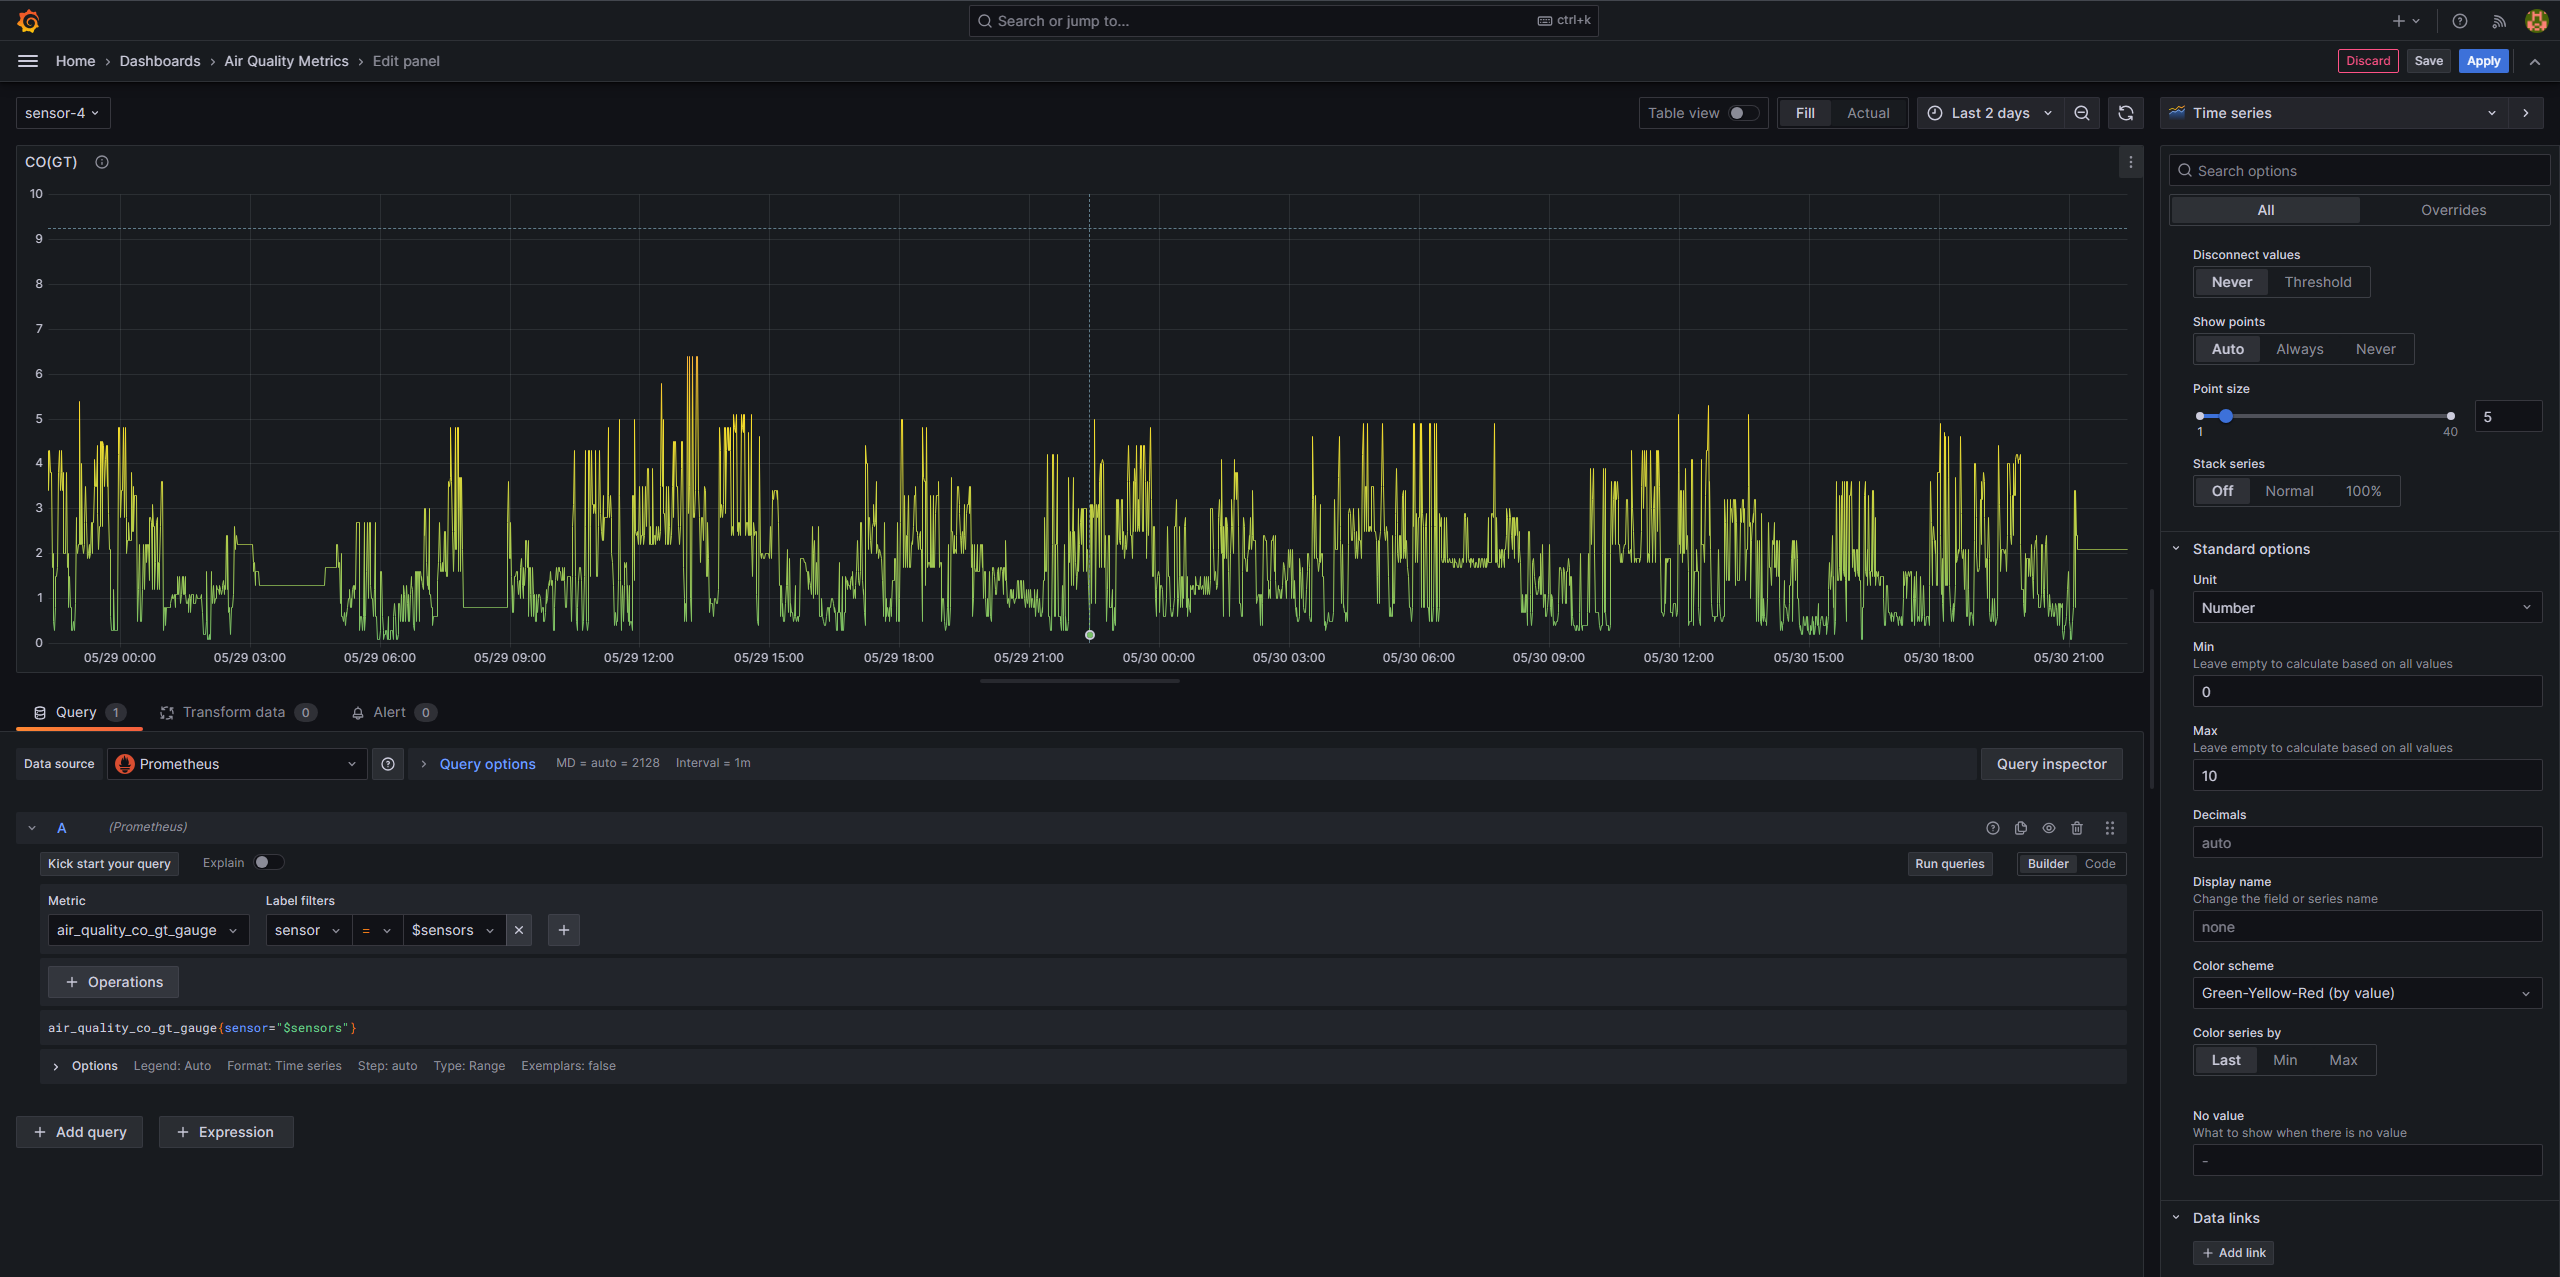
\includegraphics[width=1\textwidth]{grafana-edit-view.png}
    \centering
    \caption{Grafana visualization edit panel}
    \label{fig:graf-edit-panel}
\end{figure}

\begin{figure}[!h]
    \graphicspath{ {./screenshots/} }
    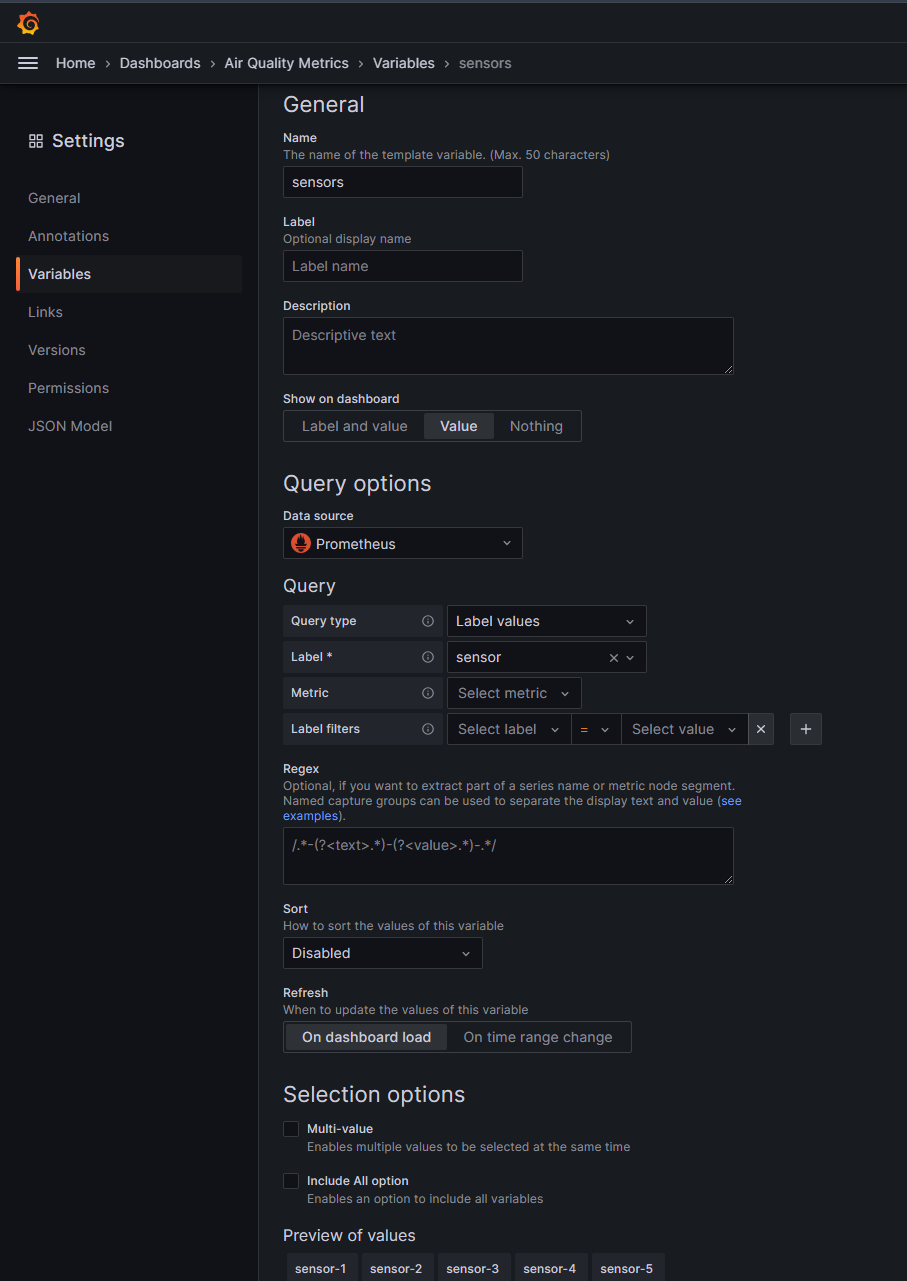
\includegraphics[width=1\textwidth]{grafana-variables-setup.png}
    \centering
    \caption{Grafana dashboard variables setup panel}
    \label{fig:graf-history-whole}
\end{figure}

\begin{figure}[!h]
    \graphicspath{ {./screenshots/} }
    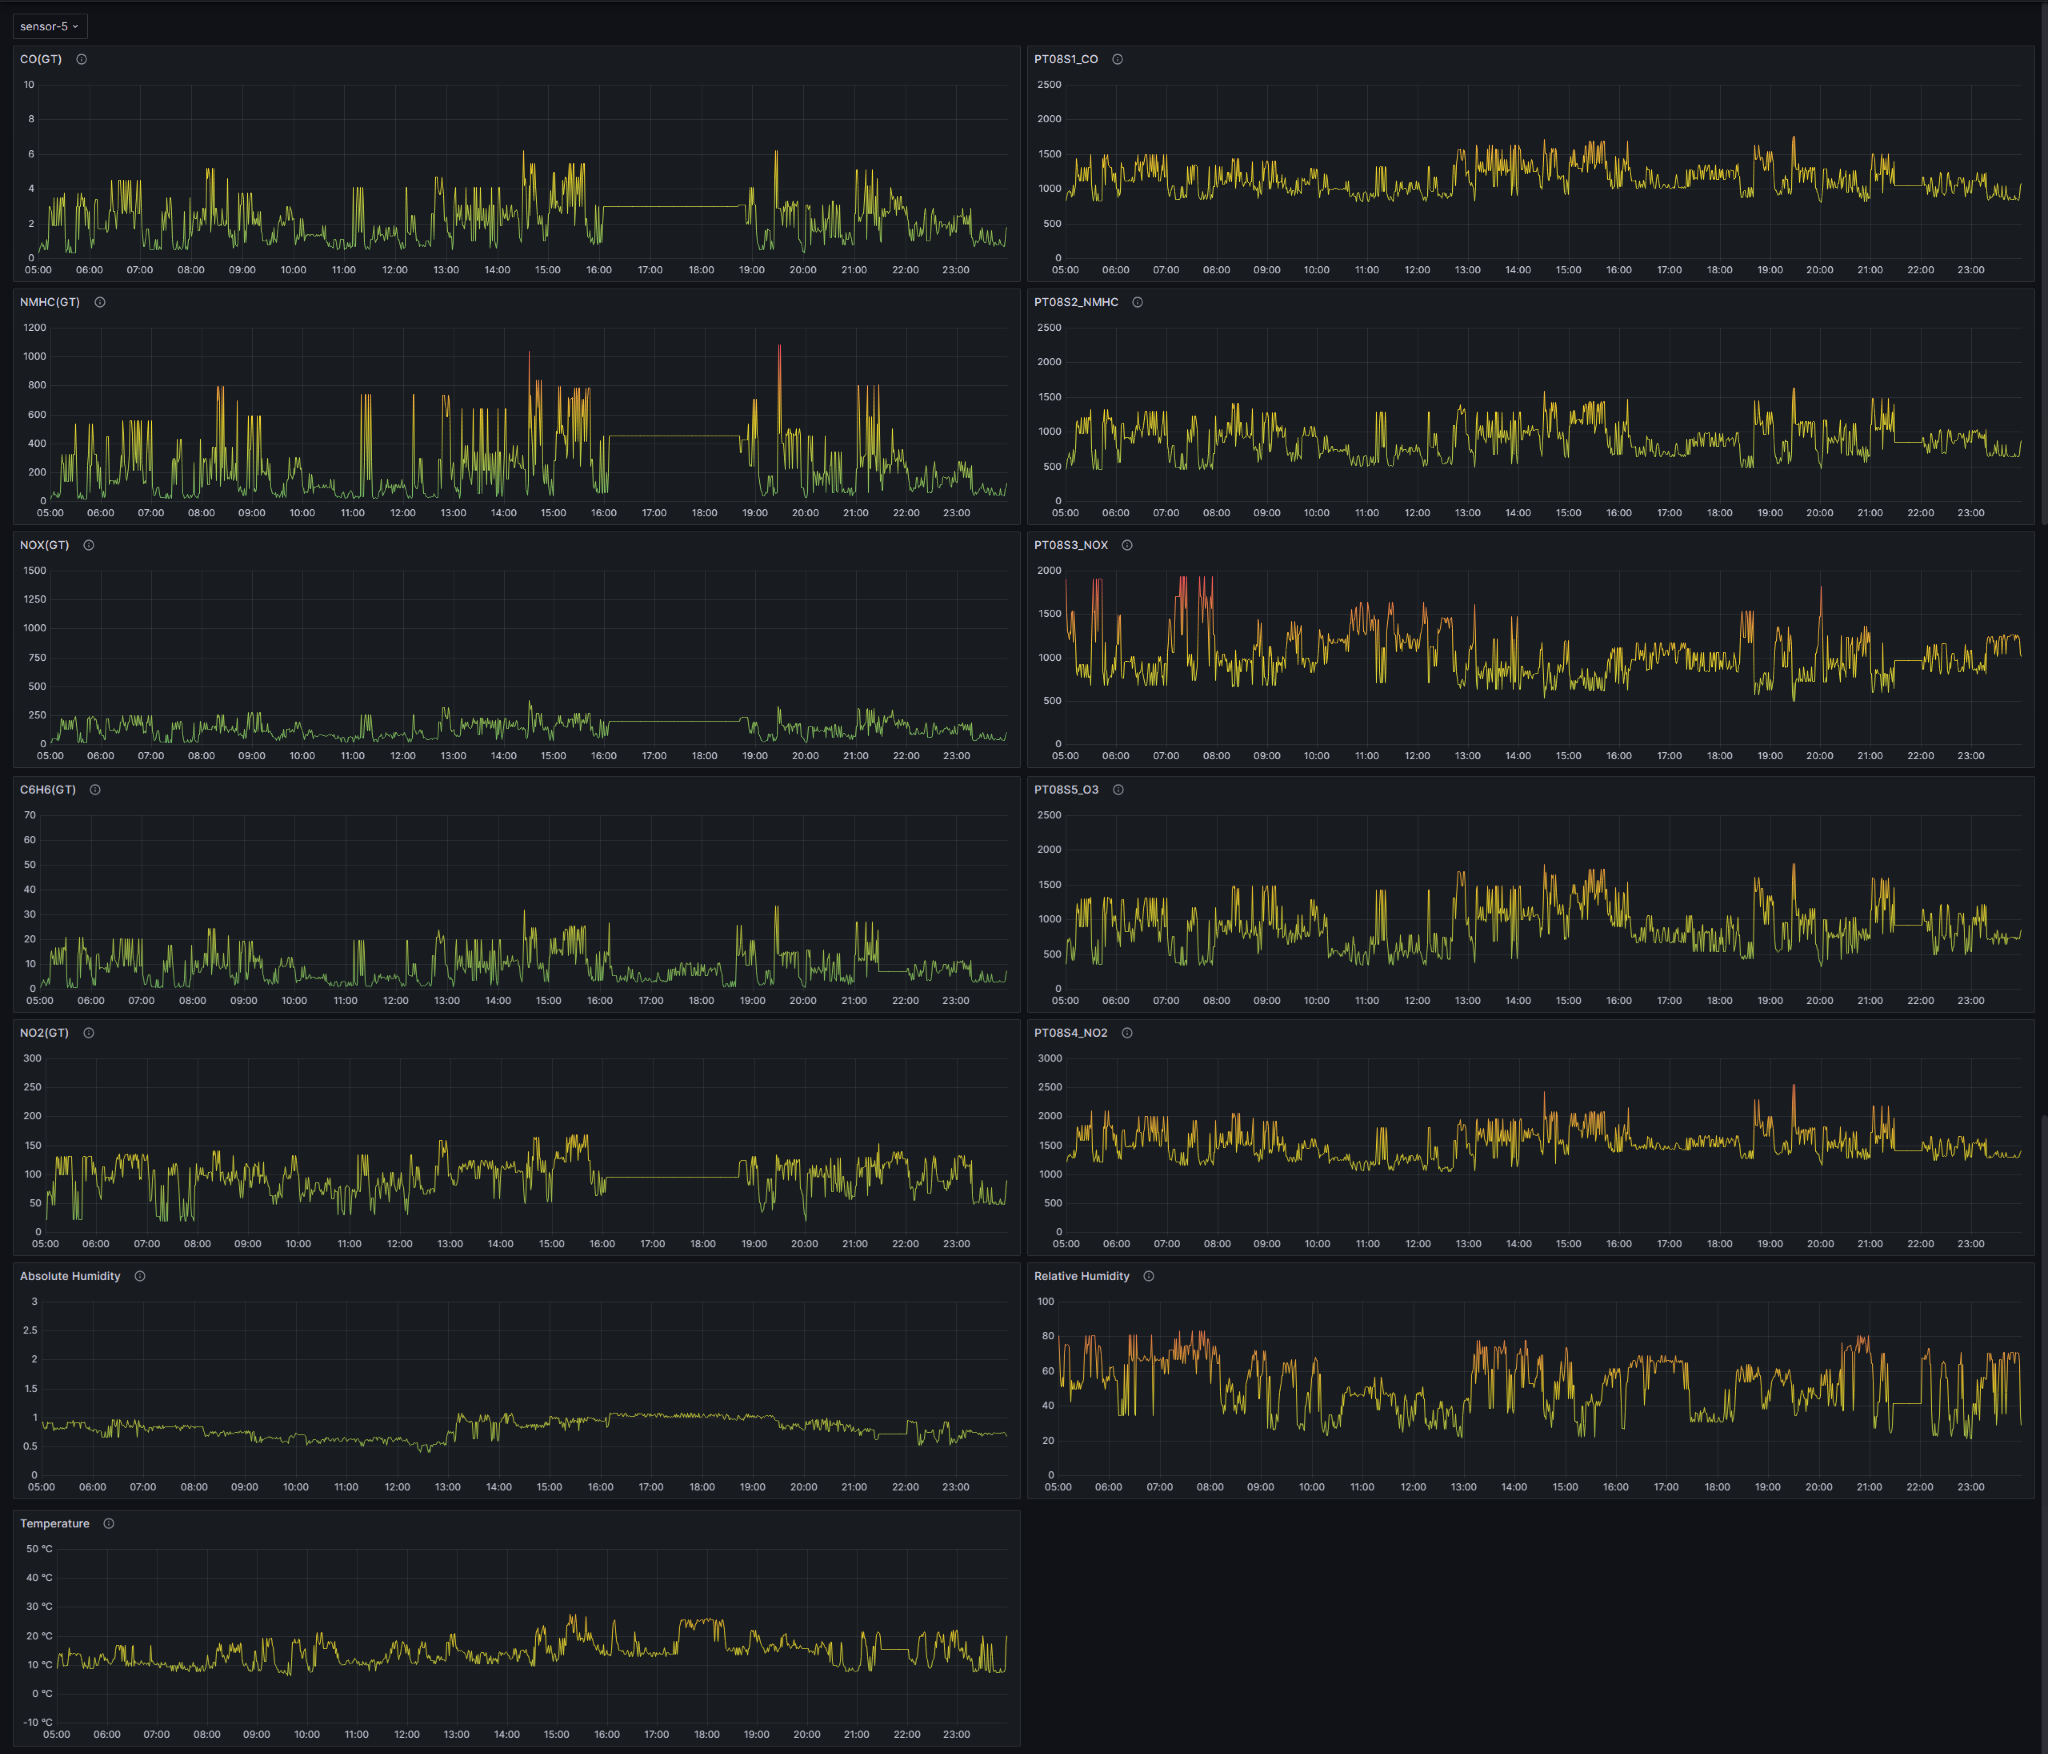
\includegraphics[width=1\textwidth]{grafana-history-whole.PNG}
    \centering
    \caption{Historical data visualizations dashboard}
    \label{fig:graf-history-whole}
\end{figure}

\begin{figure}[!h]
    \graphicspath{ {./screenshots/} }
    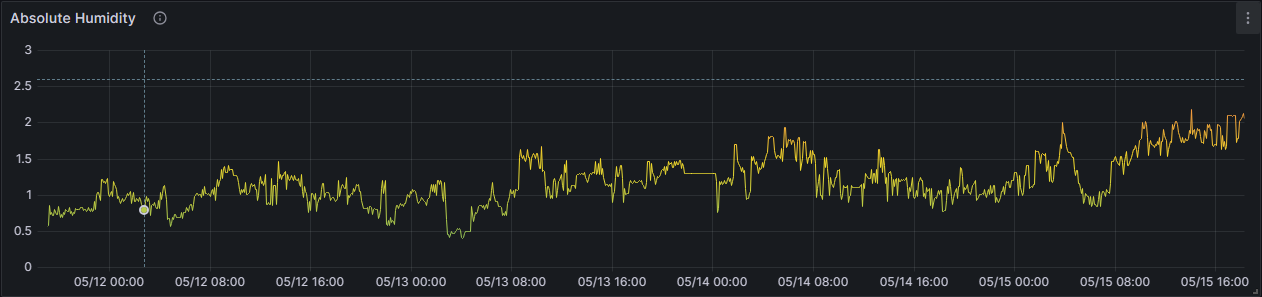
\includegraphics[width=1\textwidth]{grafana-ah.png}
    \centering
    \caption{Absolute humidity time-series visualization}
    \label{fig:graf-ah-hist}
\end{figure}

\begin{figure}[!h]
    \graphicspath{ {./screenshots/} }
    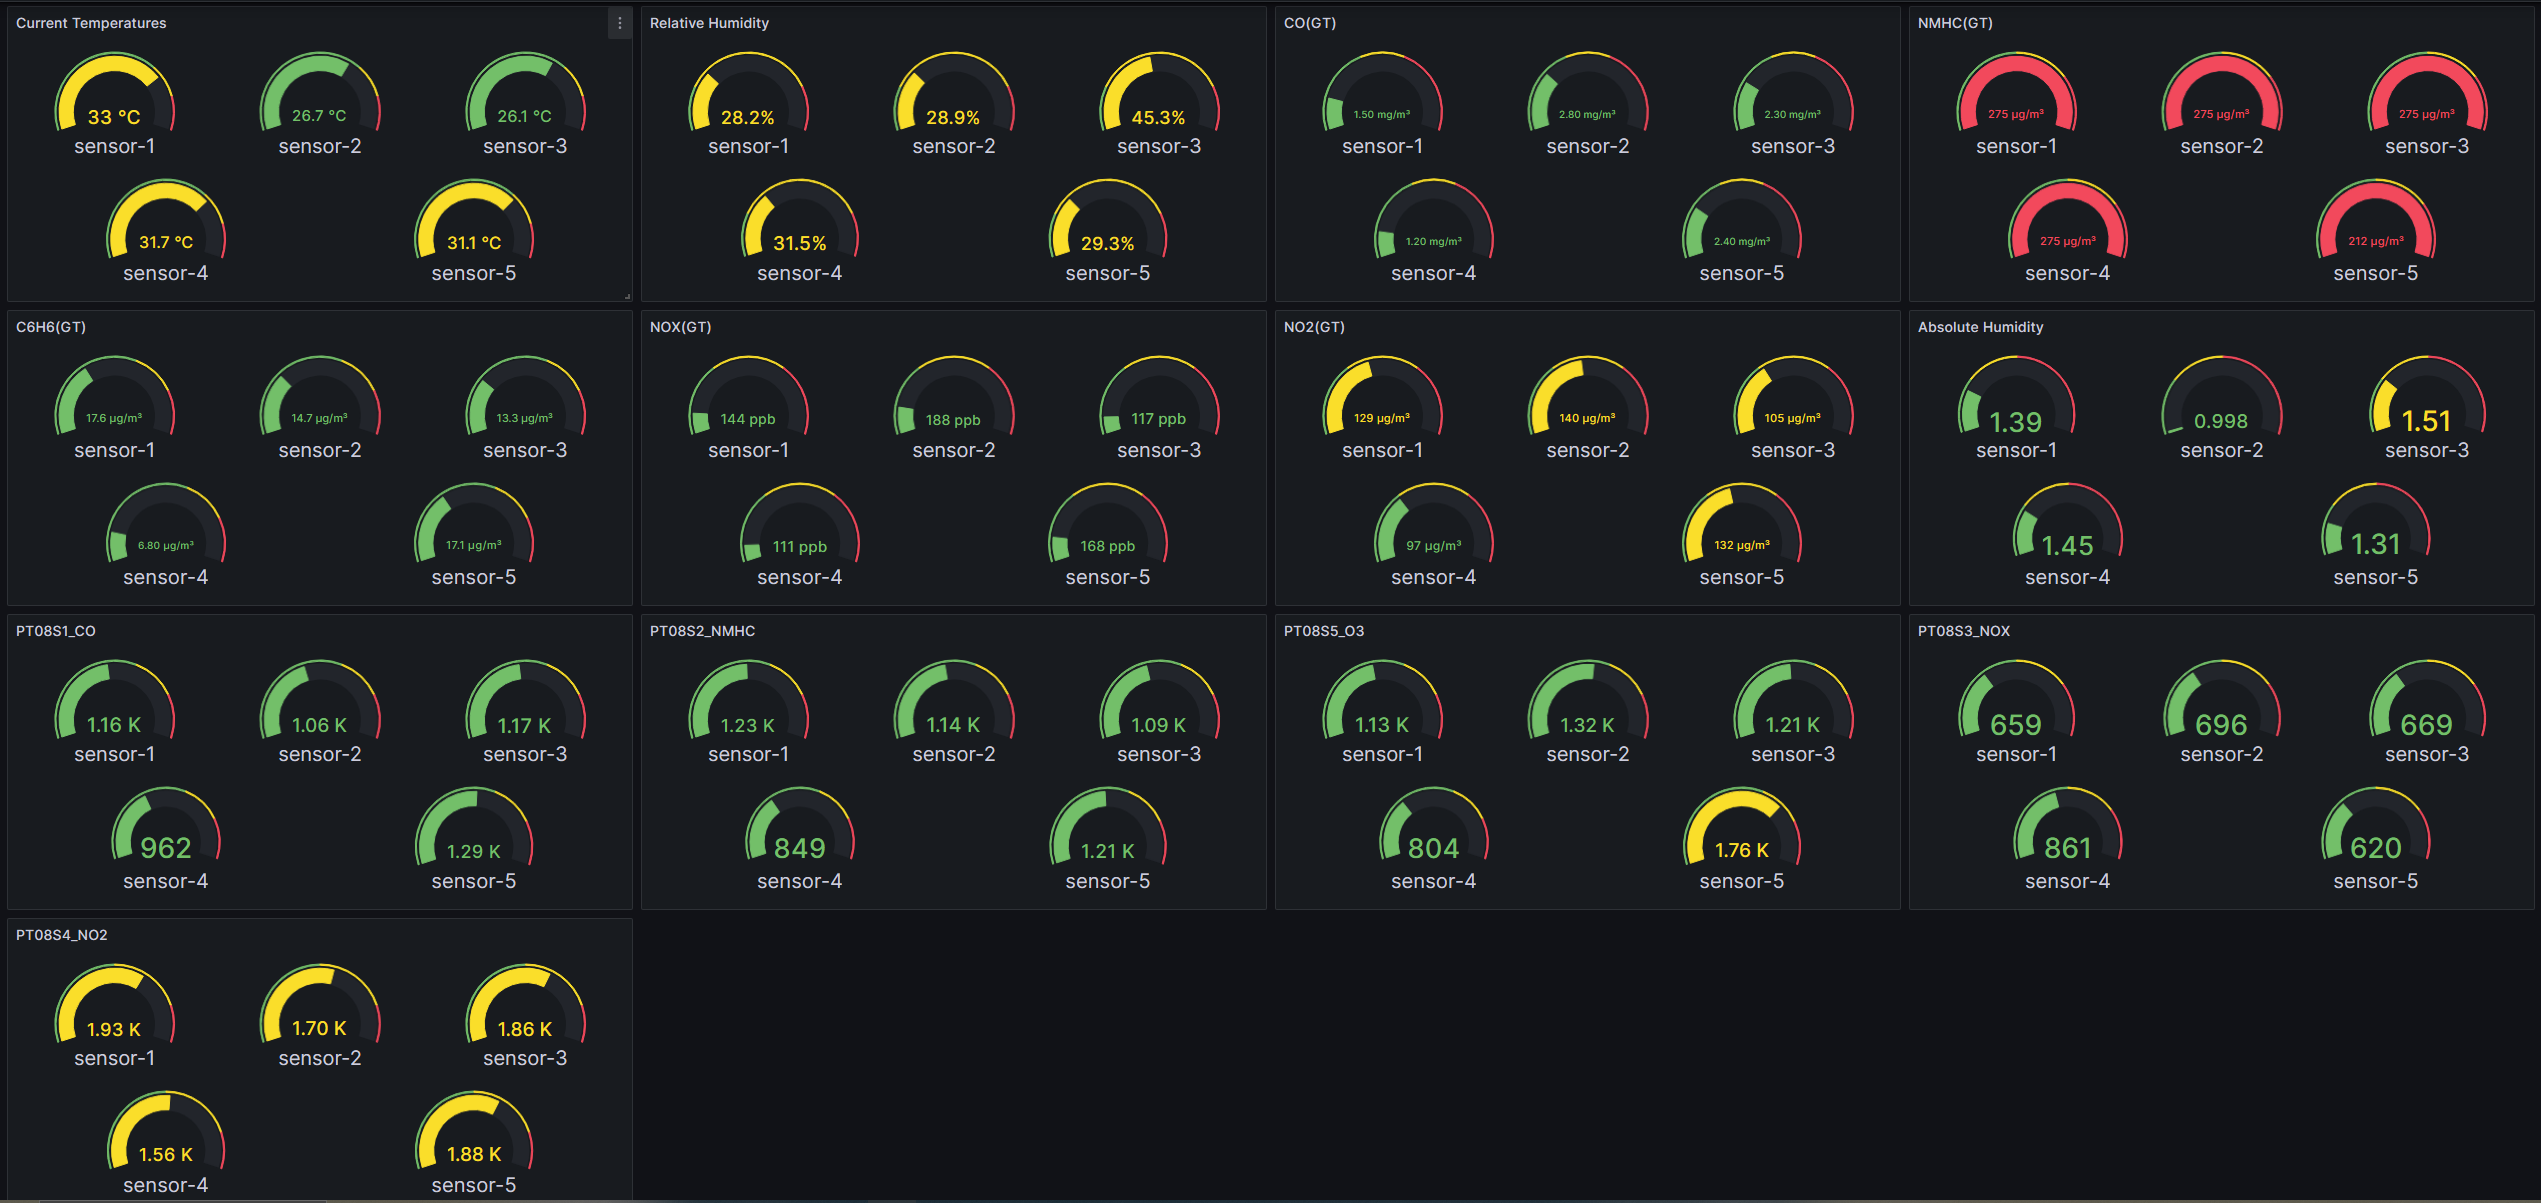
\includegraphics[width=1\textwidth]{live-whole.PNG}
    \centering
    \caption{Live value gauges dashboard}
    \label{fig:graf-live-whole}
\end{figure}

\begin{figure}[!h]
    \graphicspath{ {./screenshots/} }
    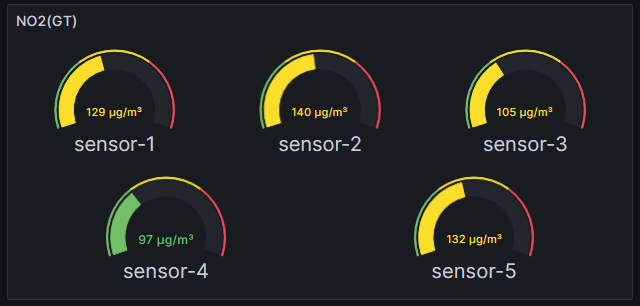
\includegraphics[width=1\textwidth]{live-nmhc.PNG}
    \centering
    \caption{Live value gauges for NMHC(GT)}
    \label{fig:graf-live-nmhc}
\end{figure}

\begin{figure}[!h]
    \graphicspath{ {./screenshots/} }
    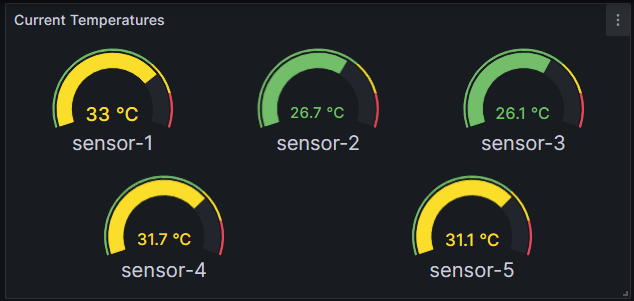
\includegraphics[width=1\textwidth]{live-temp.PNG}
    \centering
    \caption{Live value gauges for temperature}
    \label{fig:graf-live-temp}
\end{figure}

\begin{figure}[!h]
    \graphicspath{ {./screenshots/} }
    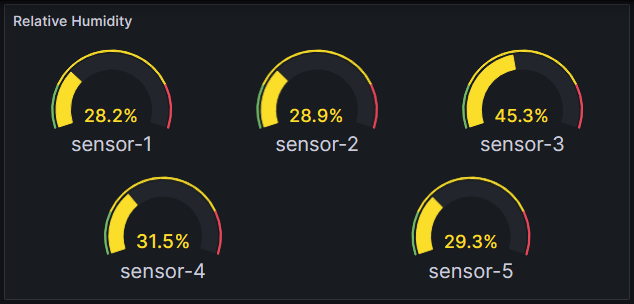
\includegraphics[width=1\textwidth]{live-rh.PNG}
    \centering
    \caption{Live value gauges for relative humidity}
    \label{fig:graf-live-rh}
\end{figure}

\FloatBarrier
\section{Orchestration}
To bring this implementation together the numerus containers created need to be deployed and orchestrated. For dynamic applications or for services requiring high availability (HA), an orchestration tool like Kubernetes could be utilized but for a static implementation like this one where a set of containers need to be deployed as a single application, Docker Compose made more sense.

Docker Compose is a tool for defining and running multi-container Docker applications using a simple YAML file. It simplifies container management by allowing defining services, networks, and volumes in a single file and spinning them up with a single command. Compared to Kubernetes, that would require setting up a cluster and defining deployments for all services/containers, Docker Compose can run on any local system equiped with Docker, making it great for local developement and small deployments.

On this implementation's Docker Compose YAML file all components, the sensors, the MQTT broker, the controller node, Prometheus and Grafana are defined as individual services, with settings such as port mapping between containers and the host machine, mounted volumes, flags, environment variables and restart policies. Also a volume for Prometheus data was defined to ensure data intergrity in case container was stopped and deleted.

\begin{minted}[%
    framesep=2mm,
    baselinestretch=1.2,
    bgcolor=LightGray,
    fontsize=\footnotesize,
    breaklines
    ]{yaml}
services:
    mqtt_broker:
        image: "eclipse-mosquitto:2.0.18"  # Using the Eclipse Mosquitto MQTT broker
        container_name: "thesis-app.mqtt_broker"
        volumes: 
        - ./mqtt_broker/mosquitto.conf:/mosquitto/config/mosquitto.conf  # Mount custom Mosquitto configuration
        ports:
        - "1883:1883"  # MQTT default port
        - "9001:9001"  # WebSockets support for MQTT
        restart: unless-stopped  # Automatically restart unless manually stopped

    exporter:
        image: "anastzampetis/iot-exporter"  # Custom IoT data exporter
        container_name: "thesis-app.exporter"
        ports:
        - "8000:8000"  # Expose exporter service on port 8000
        restart: unless-stopped  # Ensure the service restarts if it fails

    prometheus:
        image: "prom/prometheus:v2.46.0"  # Prometheus monitoring service
        container_name: "thesis-app.prometheus"
        volumes:
        - ./prometheus/prometheus.yml:/etc/prometheus/prometheus.yml  # Custom Prometheus config
        - ./prometheus/prometheus_alerts_rules.yml:/etc/prometheus/prometheus_alerts_rules.yml  # Alert rules (Empty but needed as file)
        - prometheus_data:/prometheus  # Persistent data storage
        ports:
        - "9090:9090"  # Expose Prometheus on port 9090
        command:
        - "--config.file=/etc/prometheus/prometheus.yml"  # Specify config file
        - "--web.enable-lifecycle"  # Allow configuration reload via API
        - "--storage.tsdb.path=/prometheus"  # Set data storage location
        - "--storage.tsdb.retention.time=1y"  # Retention policy. Keep data for 1 year
        restart: unless-stopped  

    grafana:
        image: "grafana/grafana:10.2.2"  # Grafana visualization service
        container_name: "thesis-app.grafana"
        ports:
        - "3000:3000"  # Expose Grafana GUI on port 3000
        restart: unless-stopped 
        environment:
        - GF_SECURITY_ADMIN_USER=admin  # Admin username for Grafana
        - GF_SECURITY_ADMIN_PASSWORD=grafana  # Admin password for Grafana
        - GF_PATHS_DATA=/var/lib/grafana  # Set data storage path
        volumes:
        - ./grafana:/var/lib/grafana  # Persist Grafana data

    # Sensor services - each sensor must be initialized separately because Docker replicas do not support dynamic variables and container names are not accessible from inside the container. (needed for MQQT client)
    sensor-1:
        image: "anastzampetis/sensor-emul"  # Custom sensor emulator image
        container_name: "thesis-app.sensor-1"
        hostname: "sensor-1"  # Set hostname for usage in the MQTT client
        restart: unless-stopped 

    sensor-2:
        image: "anastzampetis/sensor-emul"
        container_name: "thesis-app.sensor-2"
        hostname: "sensor-2"
        restart: unless-stopped

    sensor-3:
        image: "anastzampetis/sensor-emul"
        container_name: "thesis-app.sensor-3"
        hostname: "sensor-3"
        restart: unless-stopped

    sensor-4:
        image: "anastzampetis/sensor-emul"
        container_name: "thesis-app.sensor-4"
        hostname: "sensor-4"
        restart: unless-stopped

    sensor-5:
        image: "anastzampetis/sensor-emul"
        container_name: "thesis-app.sensor-5"
        hostname: "sensor-5"
        restart: unless-stopped

volumes:
    prometheus_data:  # Persistent volume for Prometheus data storage
\end{minted}

By using the above Docker Compose YAML and "docker compose up" command, all required components for this implementation are reliably instantiated with the correct configurations. This approach ensures consistency and reproducibility, making deployment seamless and error-free.

\begin{figure}[!h]
    \graphicspath{ {./screenshots/} }
    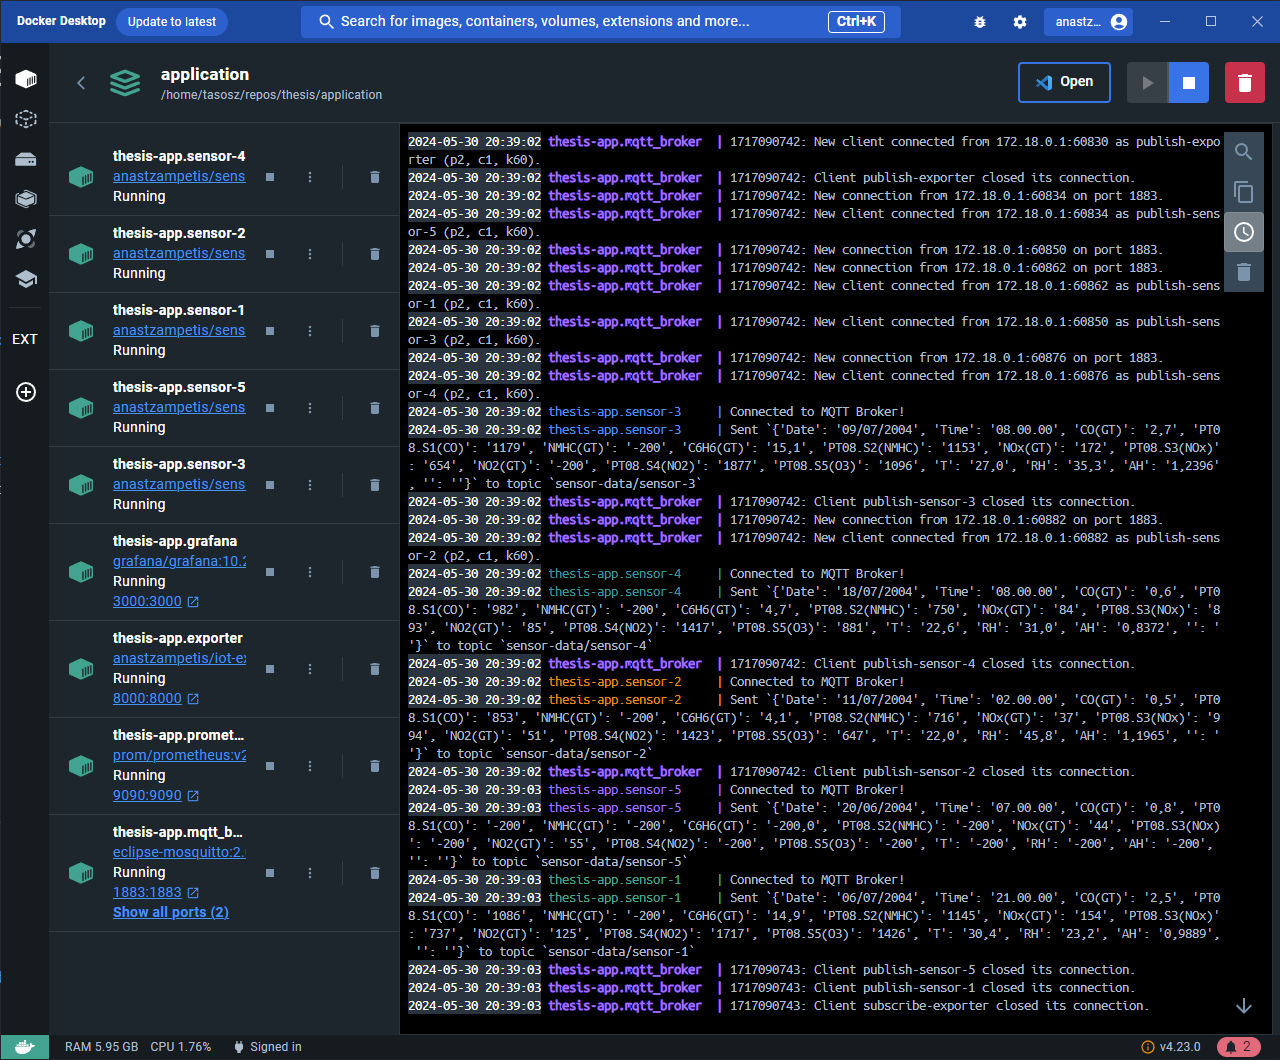
\includegraphics[width=1\textwidth]{docker_engine_compose.PNG}
    \centering
    \caption{Deployed application using Docker Compose in Docker engine's UI}
    \label{fig:docker_compose}
\end{figure}